%%%%%%%%%%%%%%%%%%%%%%%%%%%%%%%%%%%%%%%%%%%%%%%%%%%%%%%%%%%%%%%%%%%%%%%%%%%%%%%%
% AMS Beamer series / Bologna FC / Template
% Andrea Omicini
% Alma Mater Studiorum - Università di Bologna
% mailto:andrea.omicini@unibo.it
%%%%%%%%%%%%%%%%%%%%%%%%%%%%%%%%%%%%%%%%%%%%%%%%%%%%%%%%%%%%%%%%%%%%%%%%%%%%%%%%
%\documentclass[handout]{beamer}\mode<handout>{\usetheme{default}}
%
\documentclass[presentation, 9pt]{beamer}\mode<presentation>{\usetheme{AMSBolognaFC}}
%\documentclass[handout]{beamer}\mode<handout>{\usetheme{AMSBolognaFC}}
%%%%%%%%%%%%%%%%%%%%%%%%%%%%%%%%%%%%%%%%%%%%%%%%%%%%%%%%%%%%%%%%%%%%%%%%%%%%%%%%
\usepackage[T1]{fontenc}
\usepackage{wasysym}
\usepackage{amsmath,blkarray}
\usepackage[minted,most]{tcolorbox}
\usepackage{centernot}
\usepackage{fontawesome}
\usepackage{fancyvrb}
\setminted[scala]{fontsize=\scriptsize,baselinestretch=1,obeytabs=true, tabsize=2}
\usepackage[ddmmyyyy]{datetime}
\renewcommand{\dateseparator}{}
%\renewcommand{\thefootnote}{\fnsymbol{footnote}}
\newcommand{\version}{1}
\usepackage[
	backend=biber,
	citestyle=authoryear-icomp,
	maxcitenames=1,
	bibstyle=numeric]{biblatex}

	\makeatletter

\addbibresource{biblio.bib}
%%%%%%%%%%%%%%%%%%%%%%%%%%%%%%%%%%%%%%%%%%%%%%%%%%%%%%%%%%%%%%%%%%%%%%%%%%%%%%%%
\title[ScaRLib]
{ScaRLib}
%
\subtitle[]
{A Framework for Cooperative Many Agent Deep Reinforcement Learning in Scala}
%
\author[\sspeaker{Aguzzi}]
{
	\otherauthor{Davide Domini} \href{mailto:davide.domini@studio.unibo.it}{davide.domini@studio.unibo.it} \\
	\otherauthor{Filippo Cavallari} \href{mailto:filippo.cavallari@studio.unibo.it}{filippo.cavallari@studio.unibo.it} \\
	\speaker{Gianluca Aguzzi} \href{mailto:gianluca.aguzzi@unibo.it}{gianluca.aguzzi@unibo.it}\\
	\otherauthor{Mirko Viroli} \href{mailto:mirko.viroli@unibo.it}{mirko.viroli@unibo.it}
}
%
\institute[DISI, Univ.\ Bologna]
{Dipartimento di Informatica -- Scienza e Ingegneria (DISI)\\
\textsc{Alma Mater Studiorum} -- Universit{\`a} di Bologna \\[0.5cm]
\textbf{Talk @} \bold{COORDINATION 2023}}
%
\renewcommand{\dateseparator}{/}
\date[\today]{\today}
%
%%%%%%%%%%%%%%%%%%%%%%%%%%%%%%%%%%%%%%%%%%%%%%%%%%%%%%%%%%%%%%%%%%%%%%%%%%%%%%%%
\begin{document}
%%%%%%%%%%%%%%%%%%%%%%%%%%%%%%%%%%%%%%%%%%%%%%%%%%%%%%%%%%%%%%%%%%%%%%%%%%%%%%%%

%/////////
\frame{\titlepage}
%/////////

%===============================================================================
\section{Introduction}
%===============================================================================
\begin{frame}{Context}
	\centering
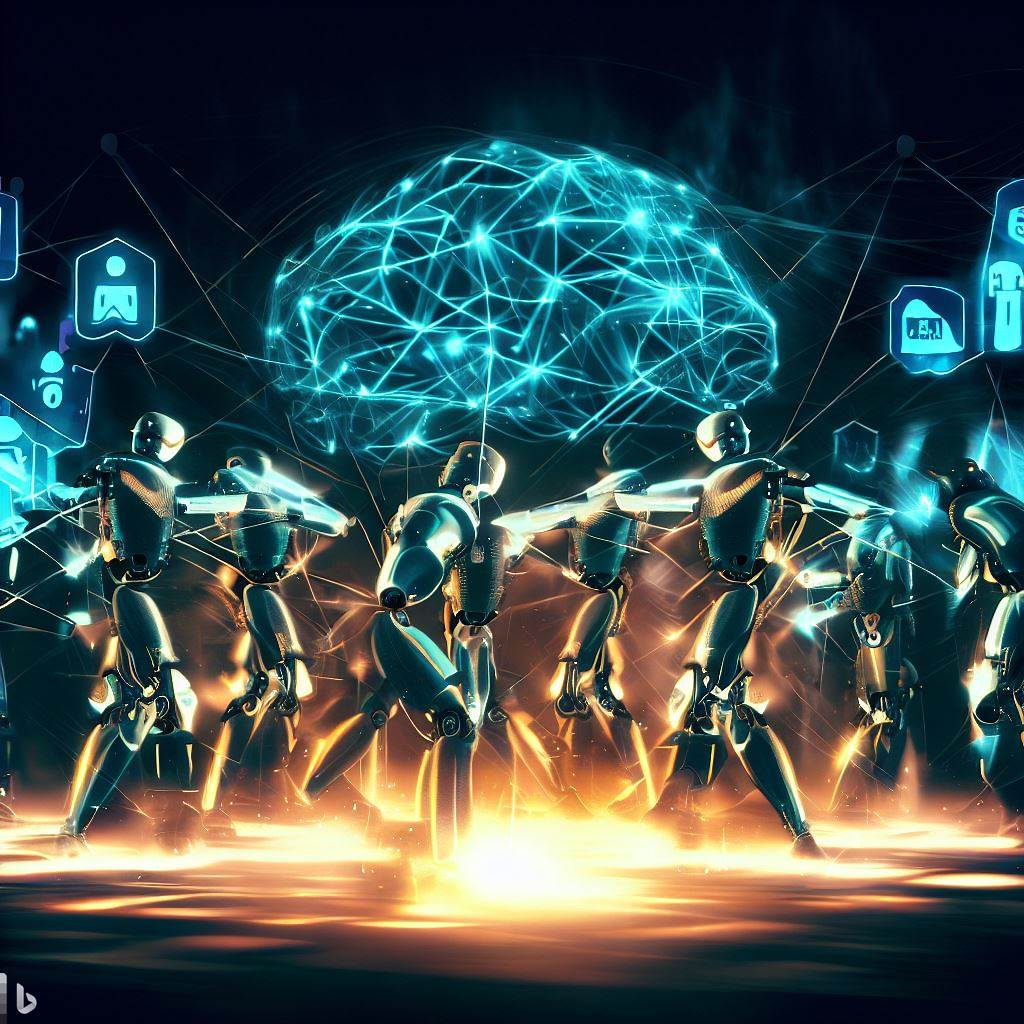
\includegraphics[width=0.5\textwidth]{img/marl.jpeg}
\\
\vspace{0.5cm}
\Large{Reinforcement Learning \faPlus \, Collective Tasks \faPlus \, Many Agent Systems}
\end{frame}
\begin{frame}{Applications}
\centering
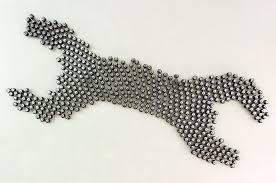
\includegraphics[height=2.35cm]{img/swarm.jpeg}
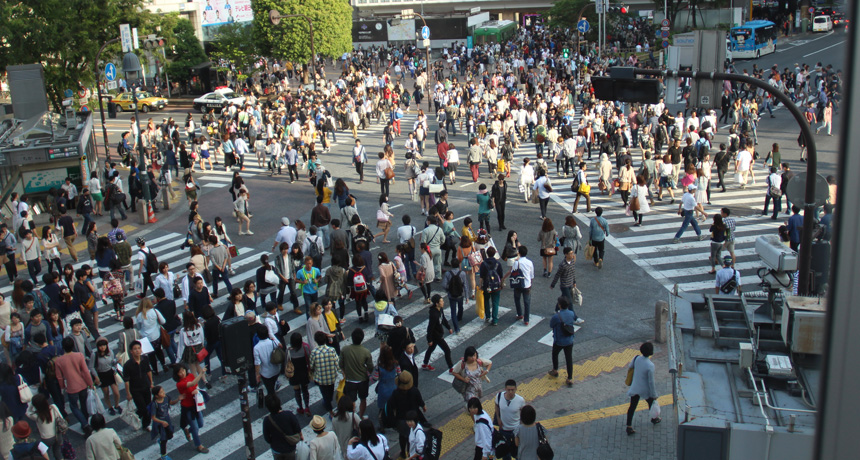
\includegraphics[height=2.35cm]{img/crowd-intersection.jpg}
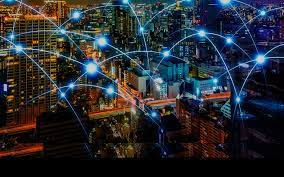
\includegraphics[height=2.35cm]{img/smart-city.jpeg}
\centering
\\
\vspace{0.12cm}
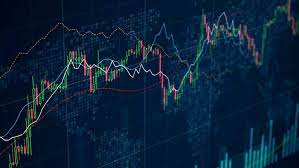
\includegraphics[height=2.35cm]{img/finance.jpeg}
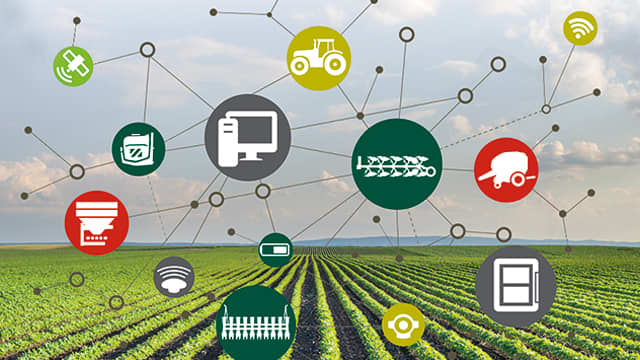
\includegraphics[height=2.35cm]{img/smart-agriculture.jpeg}
\end{frame}
\begin{frame}[allowframebreaks]{Many Agent RL -- Overview}
\begin{columns}
\begin{column}{0.55\textwidth}
	\begin{exampleblock}{Reinforcement Learning}
		\begin{itemize}
			\item \textbf{Agent} interacts with an \textbf{Environment} in \textbf{episodes} through \textbf{Actions}
			\item \textbf{Agent} learns a \textbf{Policy} to maximize  a \textbf{reward} signal 
			\item Known Algorithms (e.g., DQN, A2C, PPO, etc.)
		\end{itemize}
	\end{exampleblock}
\end{column}
\begin{column}{0.45\textwidth}
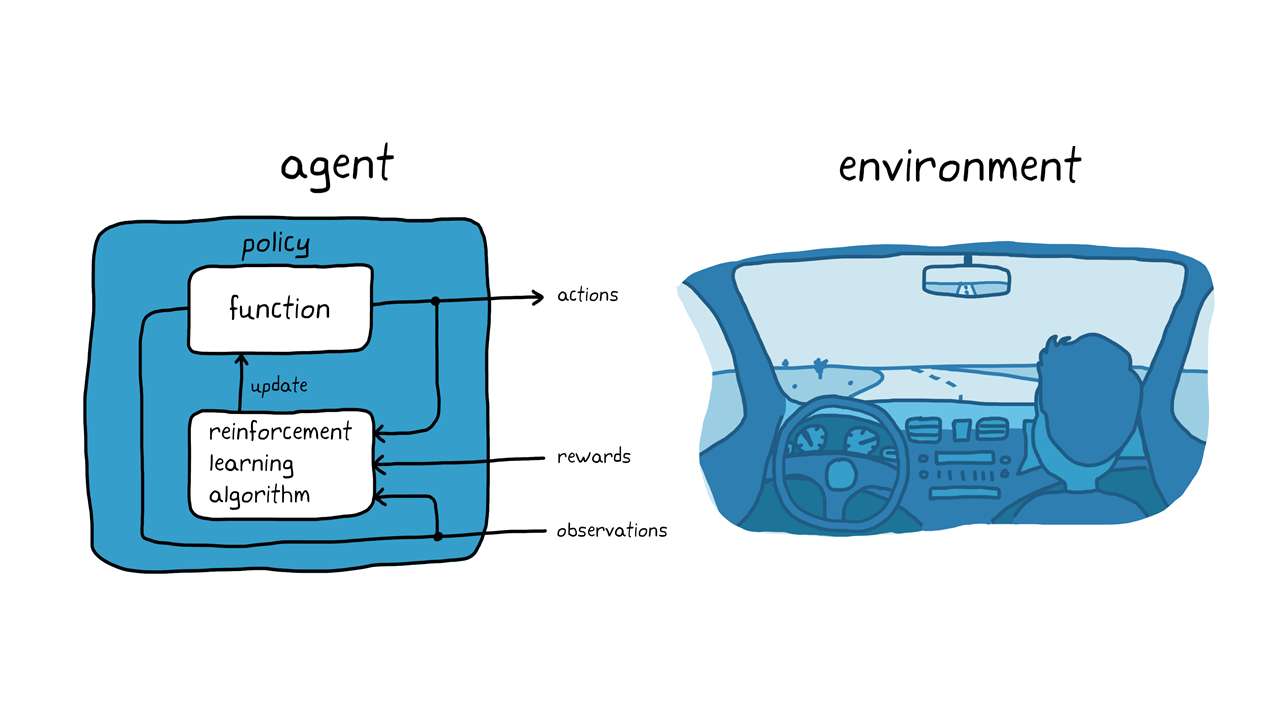
\includegraphics[width=\textwidth]{img/simple-rl.png}
\end{column}
\end{columns}

\centering
\begin{alertblock}{Many Agent RL}
\textbf{Multiple Agents} (N >> 2) interact with \textbf{shared environment} in \textbf{episodes} to maximize \textbf{global / collective reward} 
\end{alertblock}

\begin{alertblock}{Cooperative Many Agent Deep Reinforcement Learning}
   A Many Agent RL system with a \textbf{cooperative} task, sharing a \textbf{homogeneous decentralized} policy and trained in a \textbf{centralized} mode 
\end{alertblock}
\begin{exampleblock}{Task type}
	\begin{itemize}
		\item \textbf{Cooperative}: Agents cooperate to maximize global reward
		\item \emph{Competitive}: Agents compete to maximize individual reward
		\item \emph{Mixed}: Agents cooperate and compete to maximize global reward
	\end{itemize}
\end{exampleblock}

\begin{exampleblock}{Policy Type}
\begin{itemize}
	\item \emph{Centralized}: Agents share a single policy (not scalable)
	\item \textbf{Decentralized}: Agents share a set of policies (scalable)
	\begin{itemize}
		\item \textbf{Homogeneous}: Agents share the same policy
		\item \emph{Heterogeneous}: Agents use different policies
	\end{itemize}
\end{itemize}
\end{exampleblock}
\begin{exampleblock}{Training mode}
\begin{itemize}
	\item \textbf{Centralized training and decentralized execution}: Agents learn a shared policy, then use it independently
	\item \emph{Decentralized training and decentralized execution}: Agents learn a shared policy, then use it together
\end{itemize}
\end{exampleblock}
\end{frame}

\begin{frame}{Many Agent RL -- Practical concerns}
\begin{exampleblock}{Components}
	\begin{itemize}
		\item \textbf{Environment} definition: exposes API to interact with the environment and create it 
		\begin{itemize}
			\item Petting Zoo, OpenAI Gym, etc.
		\end{itemize}
		\item \textbf{Neural Network} definition: API to create and train the neural network
		\begin{itemize}
			\item PyTorch, TensorFlow, etc.
		\end{itemize}
		\item \textbf{Algorithms} implementation: exposes API to train and use the RL algorithm
		\begin{itemize}
			\item Stable Baselines, RLlib, etc.
		\end{itemize}
	\end{itemize}
\end{exampleblock}
\begin{alertblock}{Current Limitations}
	\begin{itemize}
		\item Frameworks consider only \textbf{single-agent} RL (or a few agents)
		\item Lack of abstractions for \textbf{many-agent} RL (CDTE mode, homogeneous decentralized policies, etc.)
		\item Tricky configuration of the overall training algorithms
	\end{itemize}
\end{alertblock}
\end{frame}

\begin{frame}{ScaRLib -- Overview}
\begin{exampleblock}{}
ScaRLib is a Scala framework designed to support the development of CMARL systems in JVM-based environments
\end{exampleblock}
\begin{alertblock}{Key features}
	\begin{itemize}
		\item Environment-agnostic and Neural Network-agnostic API
		\item Flexible and extensible architecture for supporting different RL algorithms/training mode
		\item Binding to state-of-the library for neural network training (e.g., PyTorch)
		\item Binding to large-scale simulator for multi-agent systems (e.g., Alchemist)
		\item Type-safe DSL for RL algorithms configuration
		\item Ready-to-use DQN implementation for homogeneous decentralized policies
		\item Integration of Aggregate computing -- a paradigm for programming large-scale distributed systems
	\end{itemize}
\end{alertblock}
\end{frame}

\begin{frame}{ScaRLib -- Project Structure}
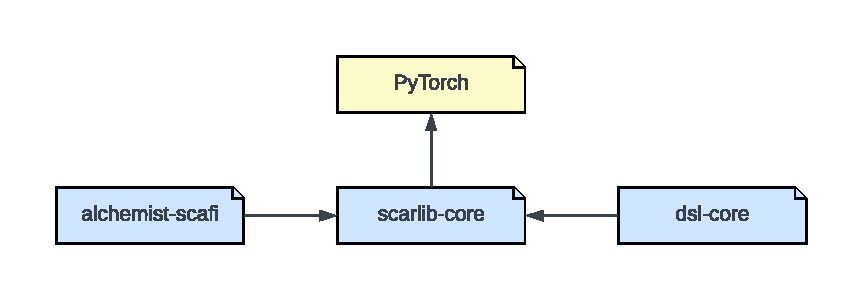
\includegraphics[width=\textwidth]{img/scarlib-modules.pdf}
\begin{itemize}
	\item \textbf{core}: Core abstractions and implementation of the framework
	\begin{itemize}
		\item Binding to PyTorch for neural network training
	\end{itemize}
	\item \textbf{alchemist-scafi}: Integration with Alchemist simulator and ScaFi
	\begin{itemize}
		\item Enable large-scale simulation of CMARL systems
	\end{itemize}
	\item \textbf{dsl-core}: Type-safe DSL for RL algorithms configuration
\end{itemize}
\end{frame}

\begin{frame}{ScaRLib -- Core}
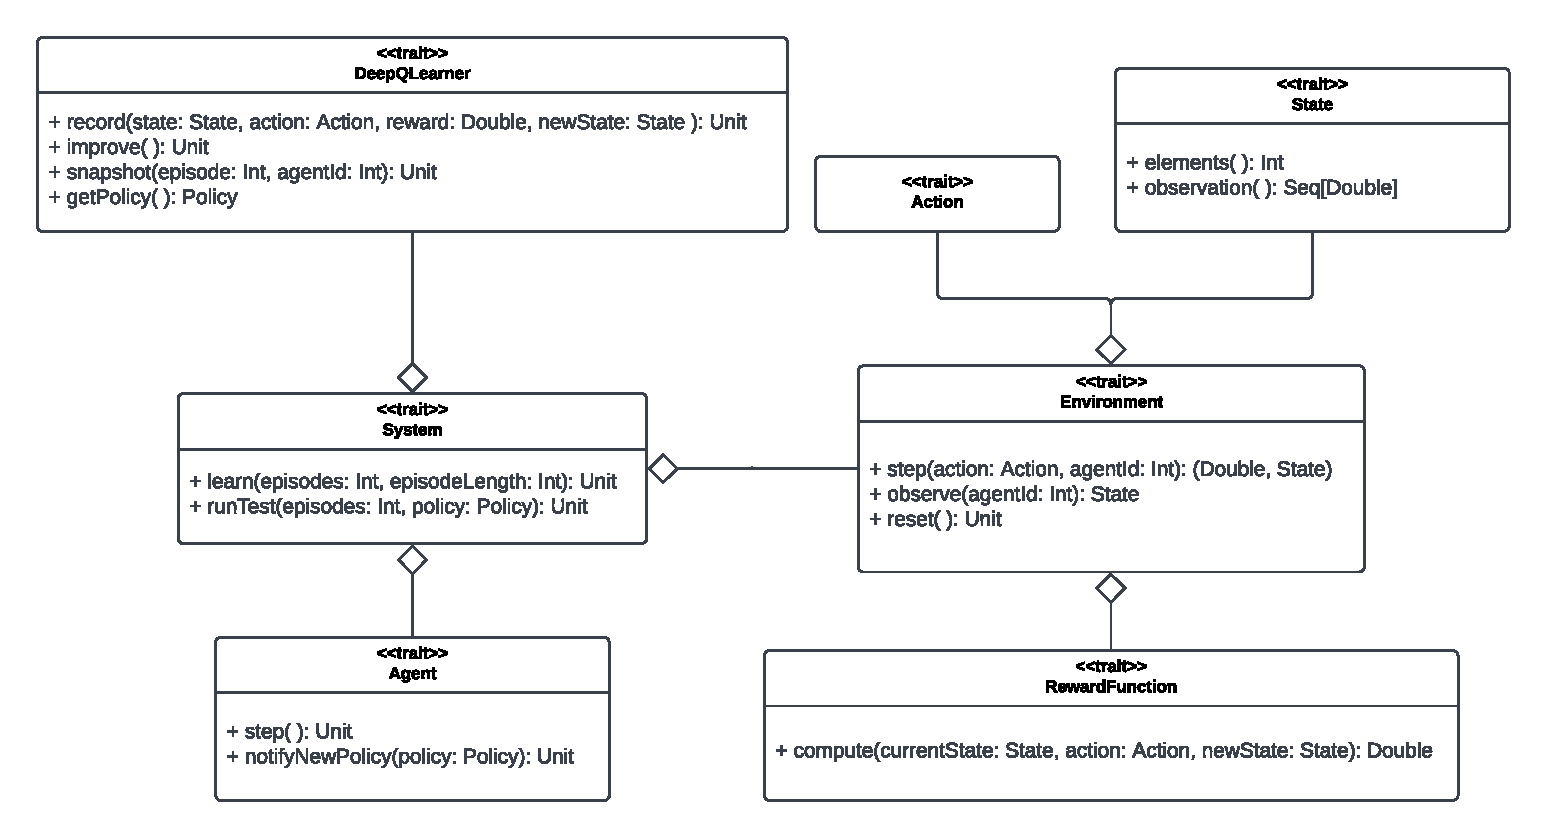
\includegraphics[width=\textwidth]{img/core-architecture.pdf}
\end{frame}

\begin{frame}{ScaRLib -- Core}
\centering
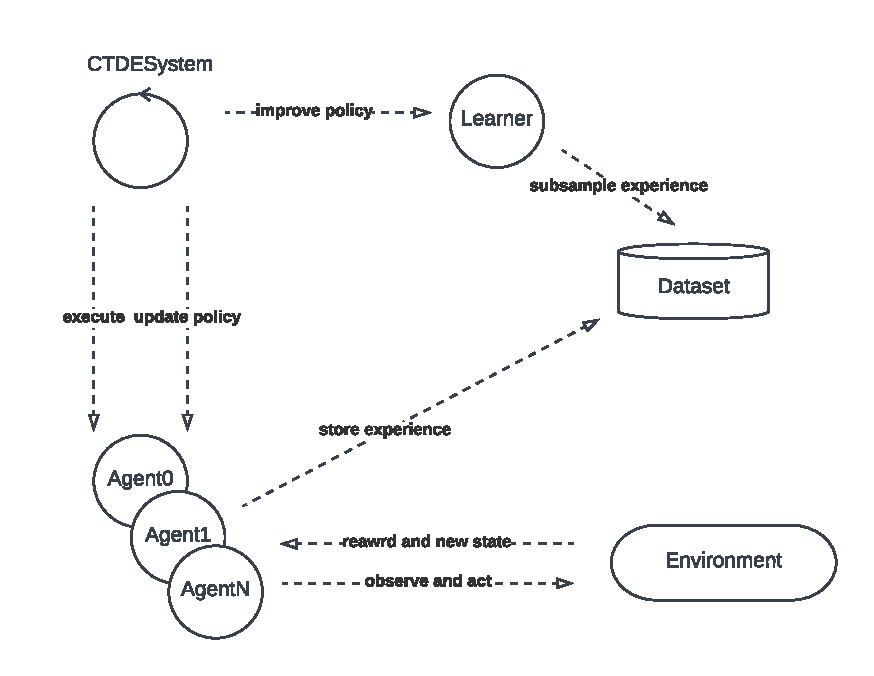
\includegraphics[width=0.8\textwidth]{img/ctdesystem.pdf}
\end{frame}
\begin{frame}{Alchemist -- In a nutshell}
Alchemist\footnote{\url{http://alchemistsimulator.github.io/}} is a simulator for pervasive, aggregate, and nature-inspired computing.

\begin{exampleblock}{Key Features}
\begin{itemize}
	\item Meta-simulator: it can express different simulation models 
	\item Used for several case studies in literatures
	\item Built-in integration with aggregate computing toolchain
\end{itemize}
\end{exampleblock}
\centering
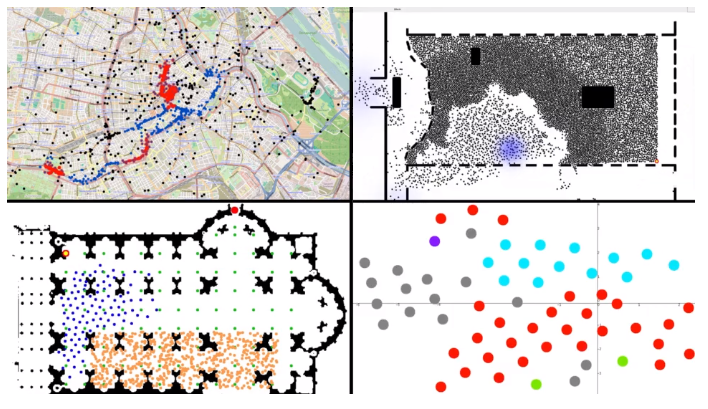
\includegraphics[width=0.6\textwidth]{img/alchemist}

\end{frame}
\begin{frame}{ScaFi -- In a nutshell}
ScaFi (Scala Fields) is a Scala-based library and framework for Aggregate Programming.
\begin{exampleblock}{Key Features}
	\begin{itemize}
		\item DSL for field calculus 
		\item Support of a akka-based middleware for distributed execution
		\item Web playground to test and debug aggregate computing programs
		\item Binding to Alchemist simulator for large-scale simulation
	\end{itemize}
\end{exampleblock}
\centering
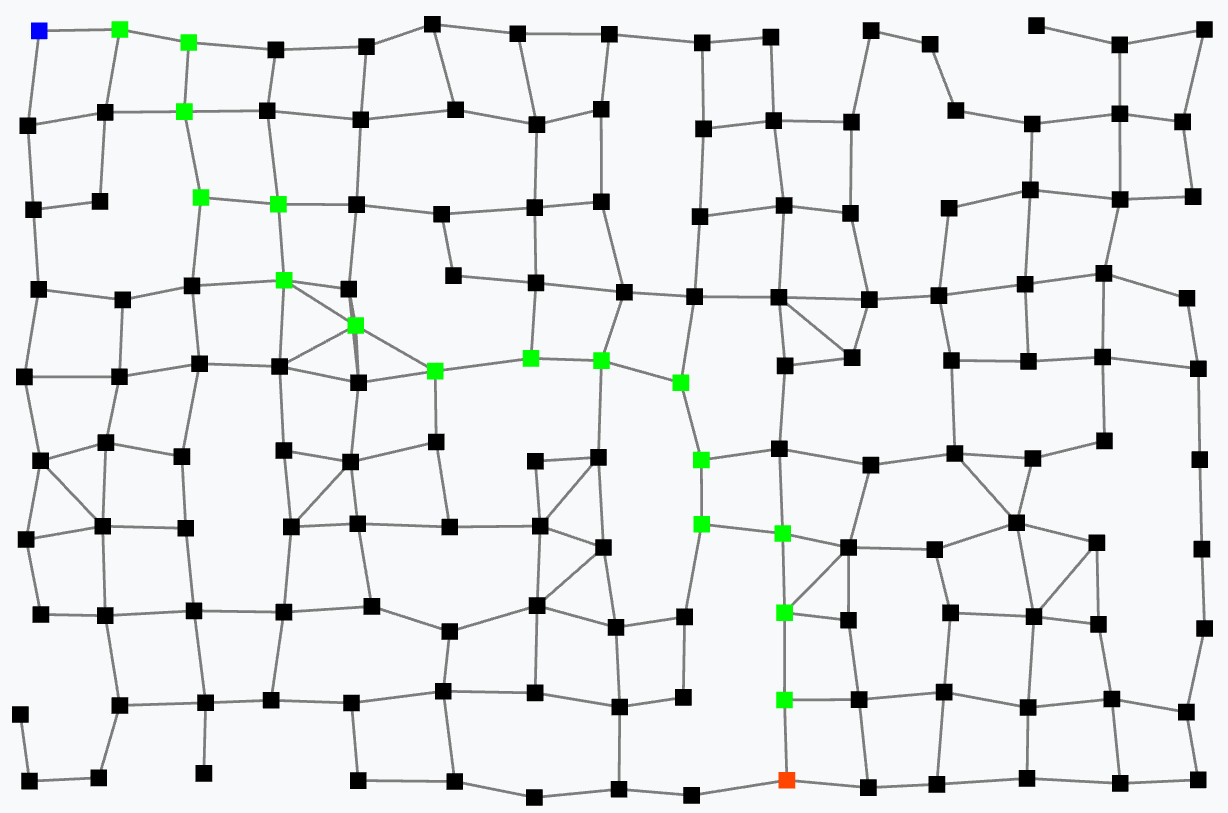
\includegraphics[width=0.5\textwidth]{img/channel.png}
\end{frame}
\begin{frame}{ScaRLib -- Alchemist ScaFi Integration}
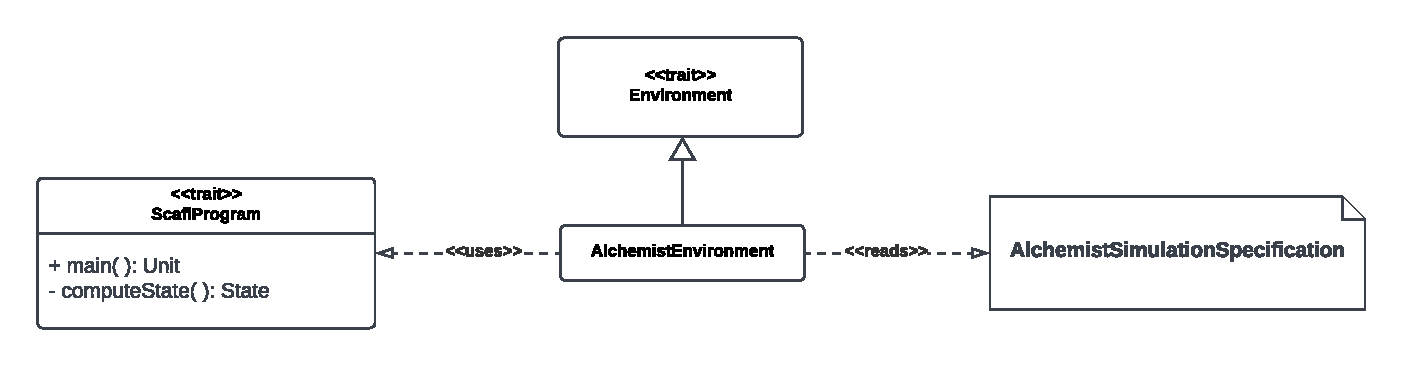
\includegraphics[width=\textwidth]{img/alchemist-scafi-arc.pdf}
\begin{itemize}
	\item \textbf{AlchemistEnvironment}: facade for alchemist simulation specified through a configuration file
	\item \textbf{ScaFiProgram}: aggregate computing program to be executed by Alchemist that computes the state of the agent
\end{itemize}
\end{frame}
\begin{frame}[fragile]{ScaRLib -- DSL}
\begin{itemize}
	\item Simplify the creation of a learning system guiding the user with types
	\item It supports the definition of different training modes (DTDE or CTDE) and it is possible to express the main components of a learning system (e.g., reward function, dataset, etc.)
\end{itemize}
\centering
\begin{minted}[fontsize=\small, frame=single]{scala}
val system = learningSystem {
	rewardFunction { new MyRewardFunction() }
	actions { MyAction.all }
	dataset { ReplayBuffer[State, Action](10000) }
	agents { 50 } // select the number of agent
	environment {
		// select a specific environment
		"it.unibo.scarlib.experiments.myEnvironment"
	}
}
\end{minted}
\end{frame}
\begin{frame}{Experiments: Learn to Flock}
\begin{exampleblock}{Description}
	\begin{itemize}
		\item Agents must learn to flock in a 2D environment
		\item The state is composed of the directions of the agents within the field of view of the agent
		\item The reward function balance the collision versus the cohesion of the agents
	\end{itemize}
\end{exampleblock}
\begin{alertblock}{Implementation}
	\begin{itemize}
		\item The environment is based on an Alchemist simulation
		\item The state is computed by a ScaFi program
		\item The policy is a DQN with a fully connected neural network with 2 hidden layers
		\item The training is performed in CTDE mode with 50 agents for 1000 episodes
		\item Then we evaluated the policy in different agent population
	\end{itemize}
\end{alertblock}
\end{frame}

\begin{frame}{Experiment: Results}
\centering
\fbox{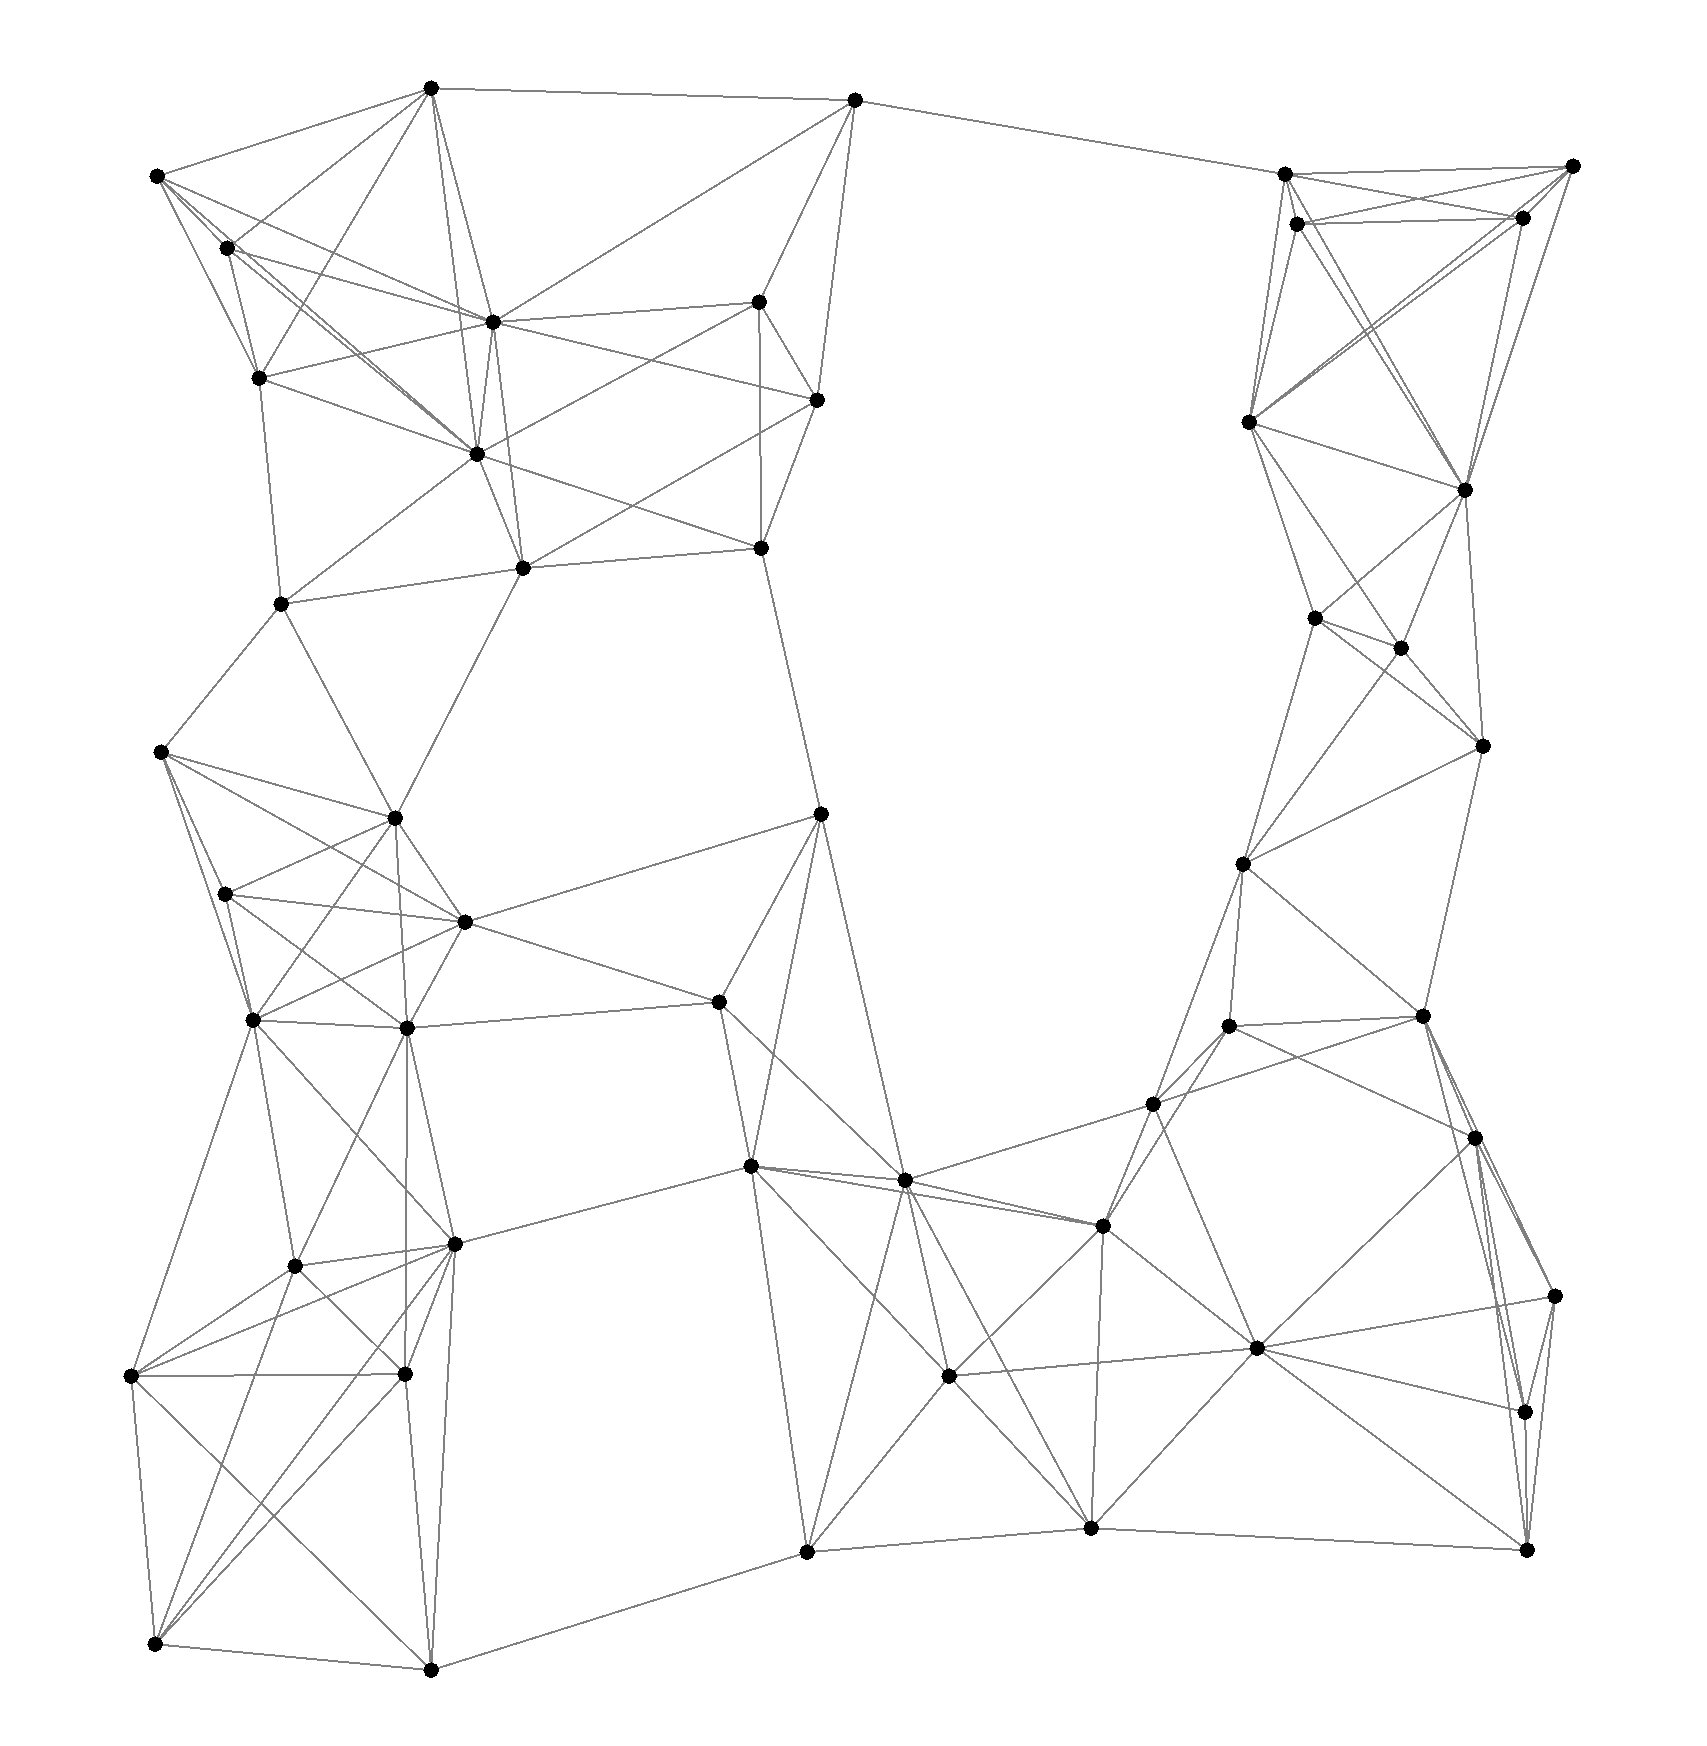
\includegraphics[width=0.25\textwidth]{img/1.png}}
\fbox{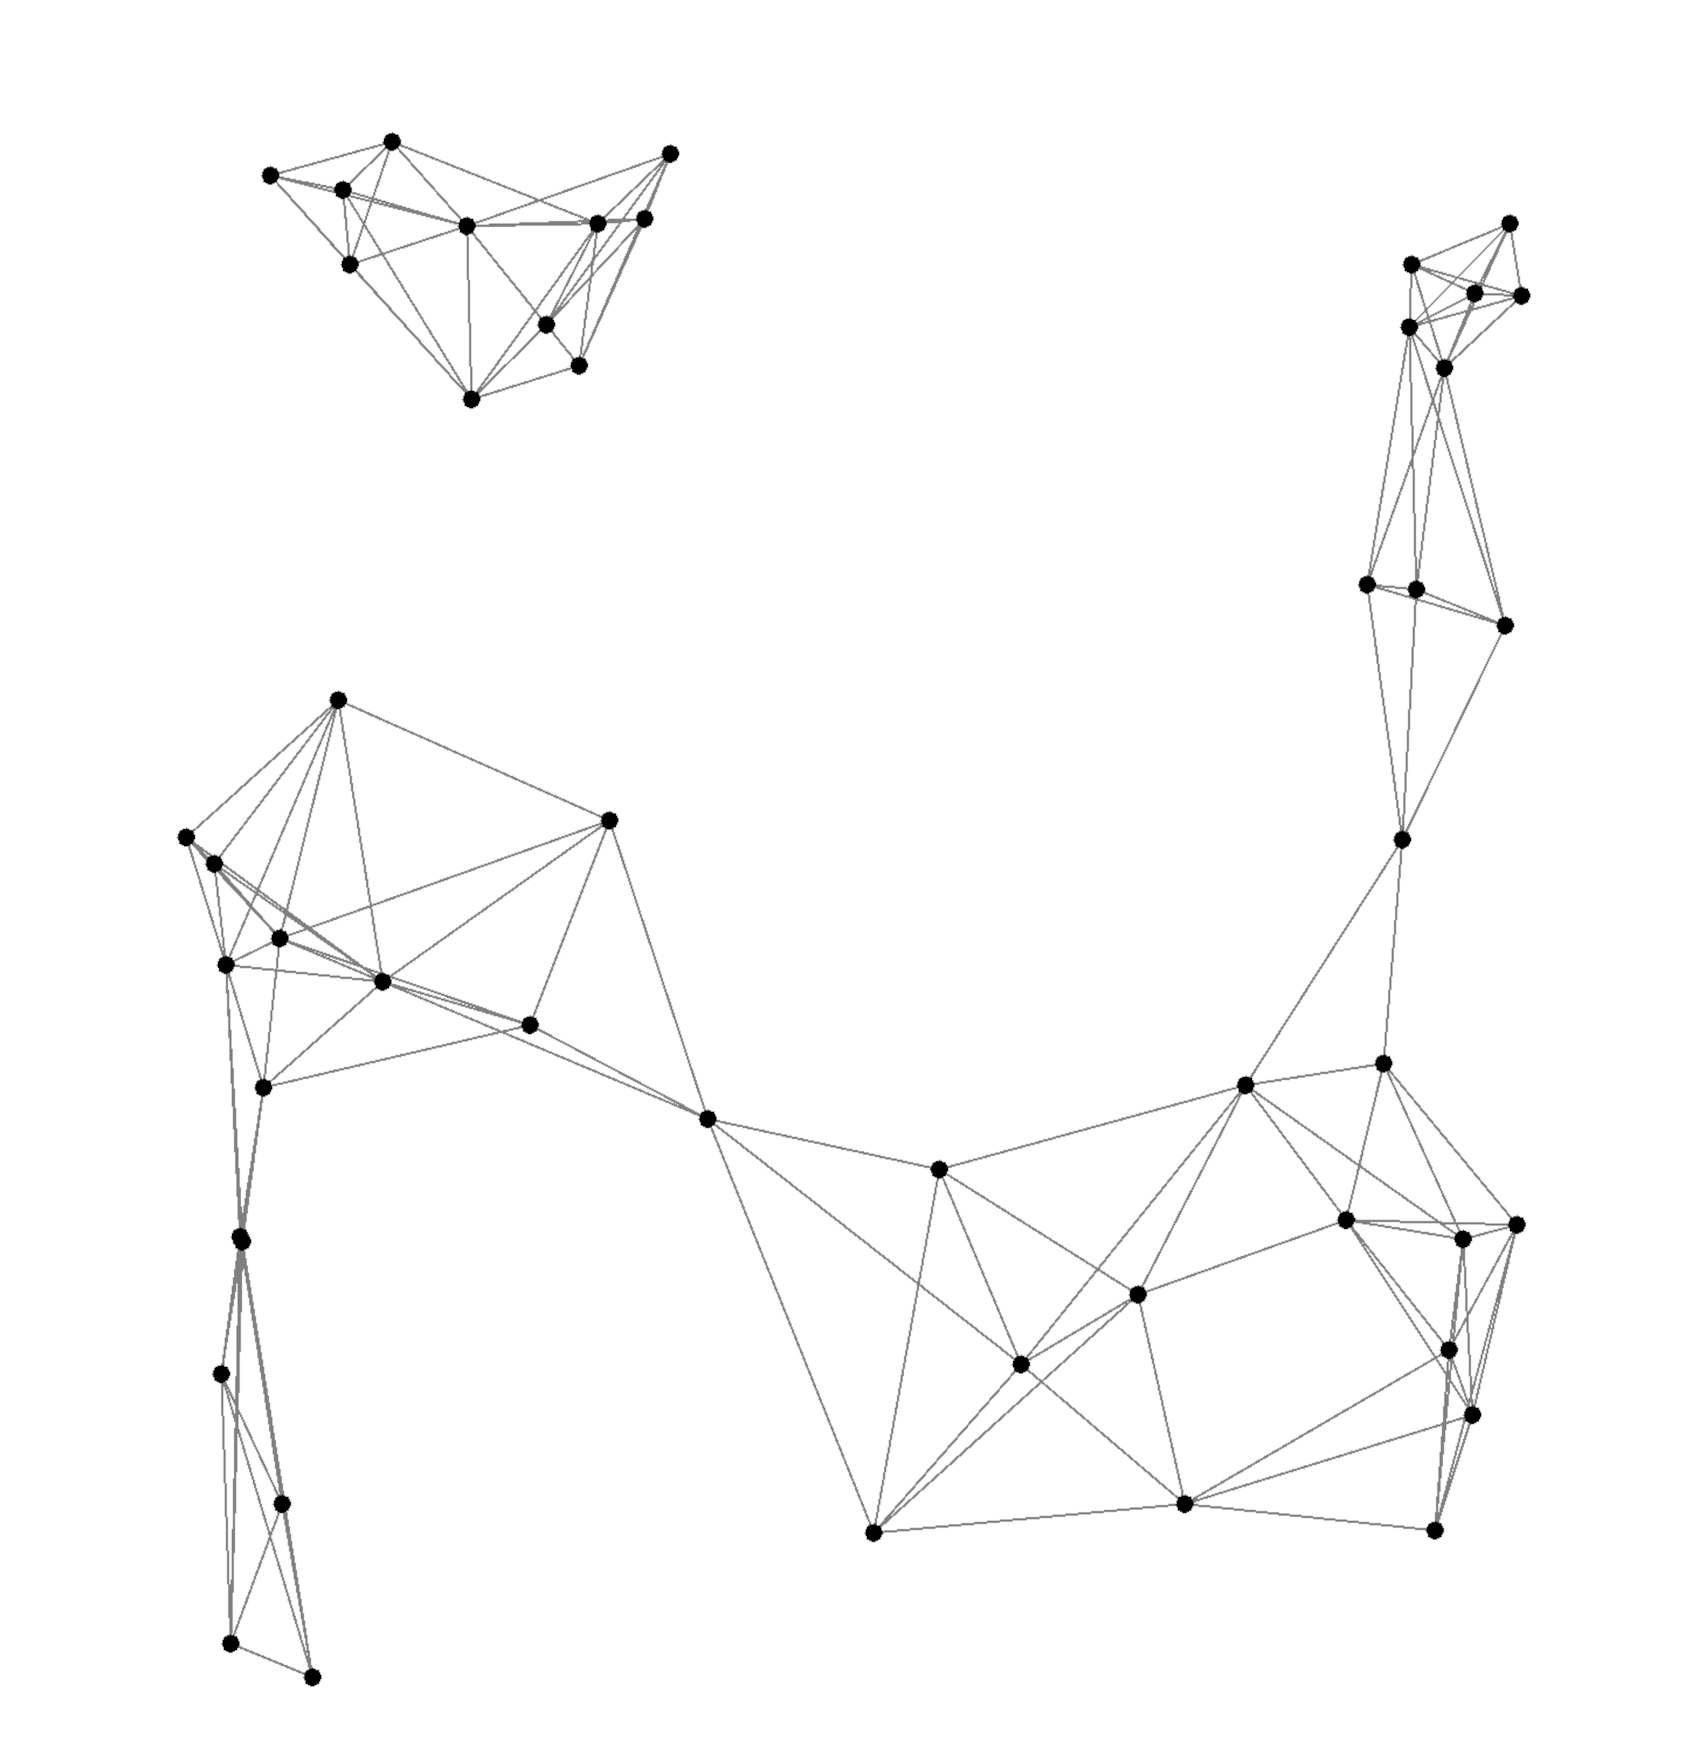
\includegraphics[width=0.25\textwidth]{img/4.png}}
\fbox{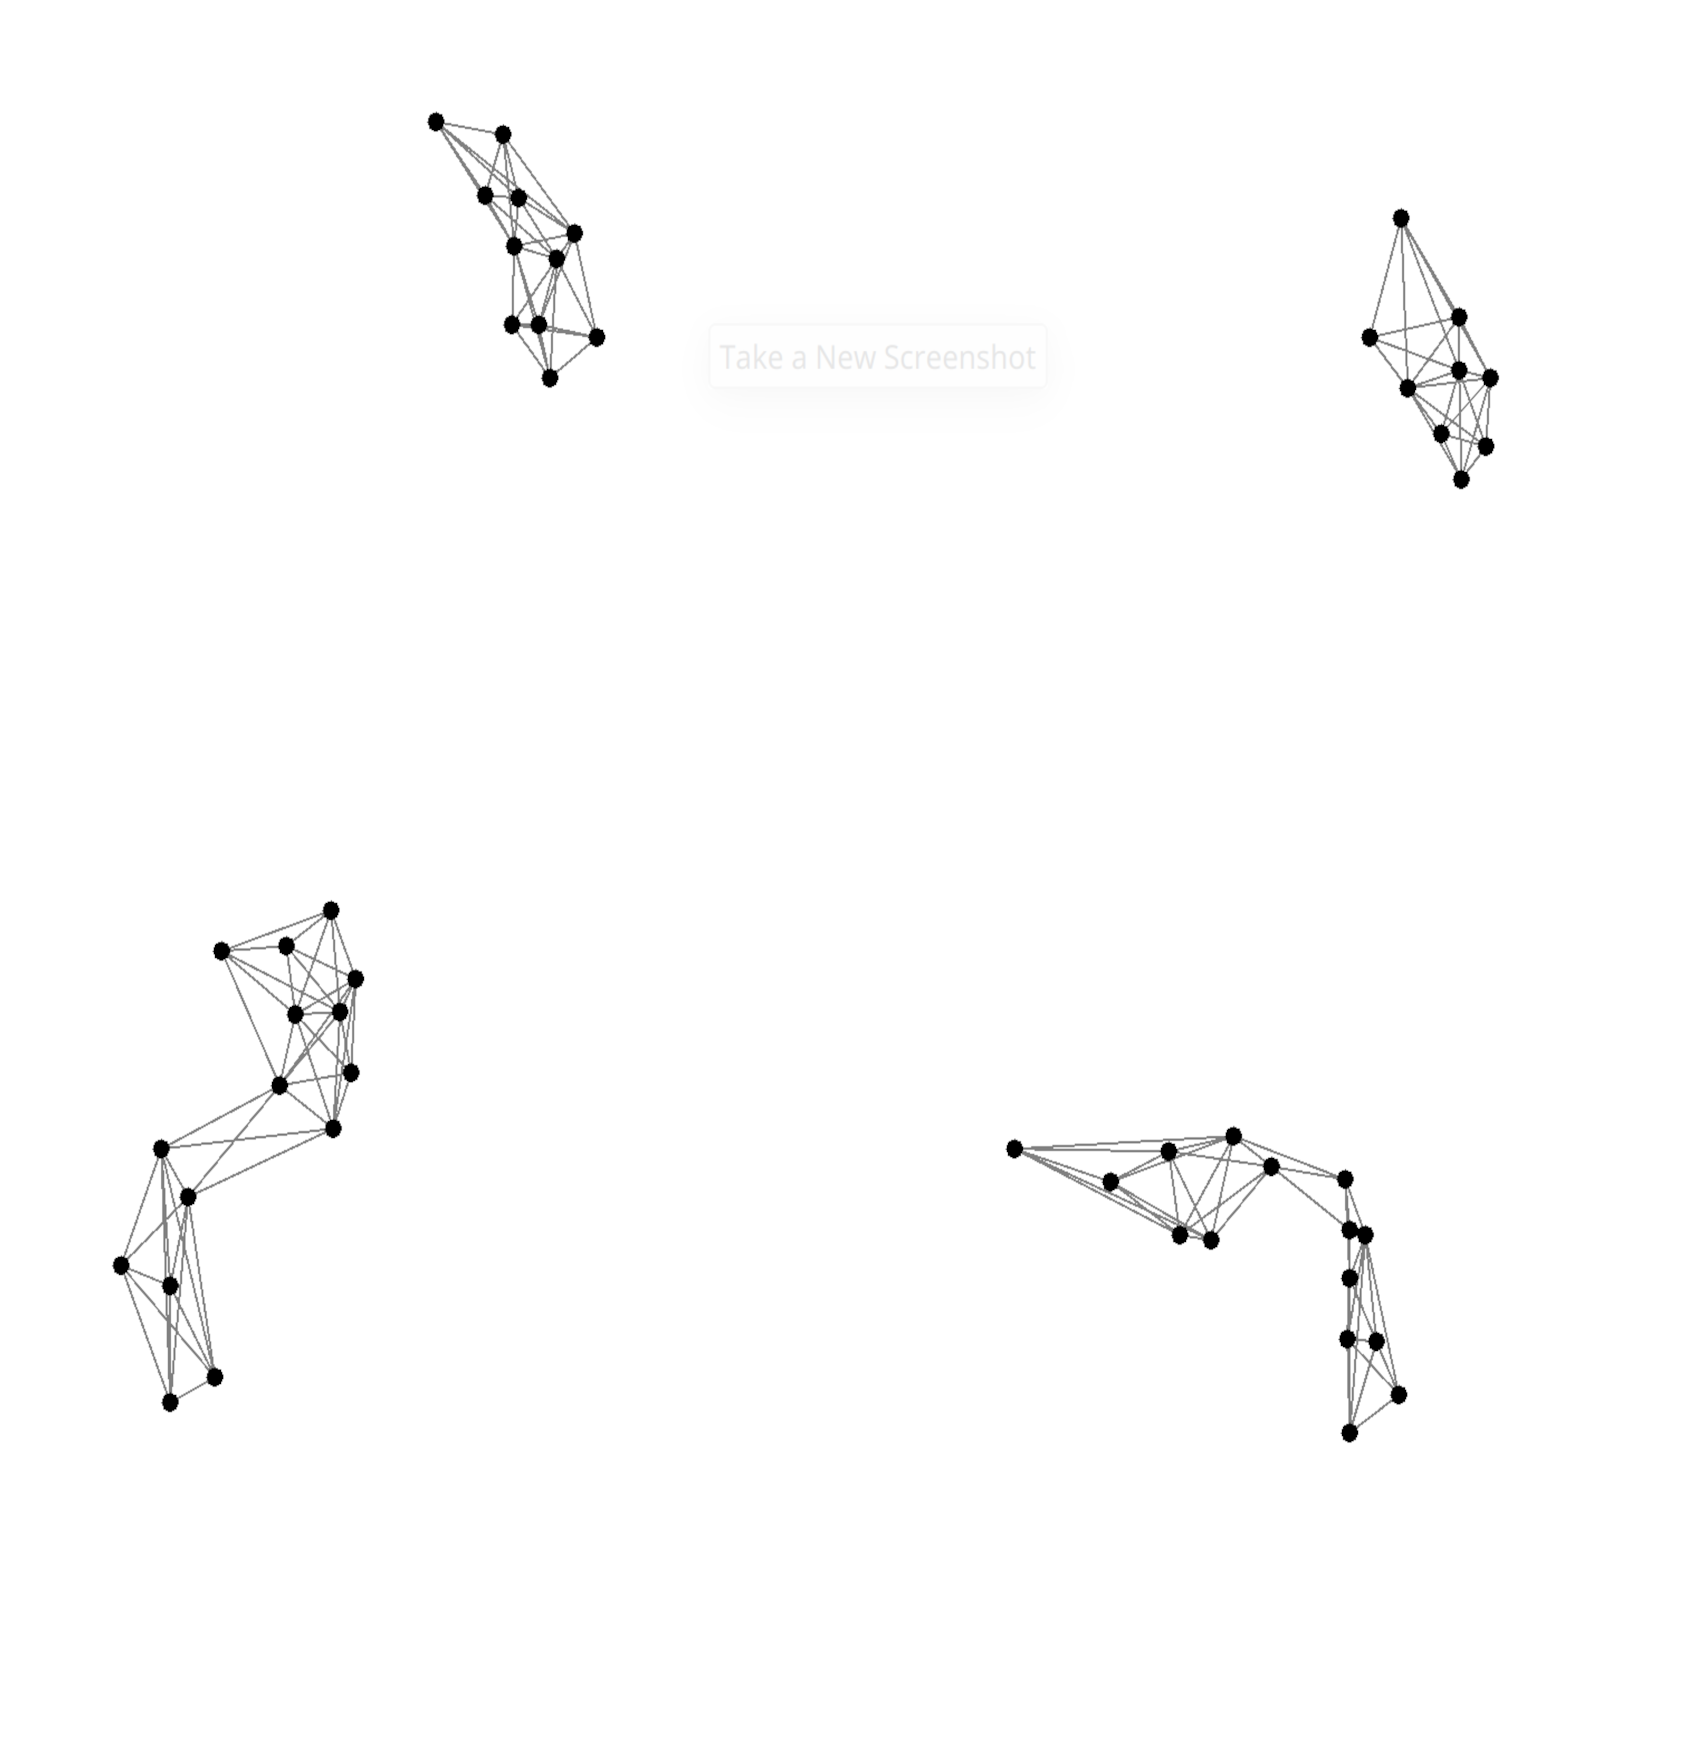
\includegraphics[width=0.25\textwidth]{img/7.png}}

\vspace{0.1cm}
\fbox{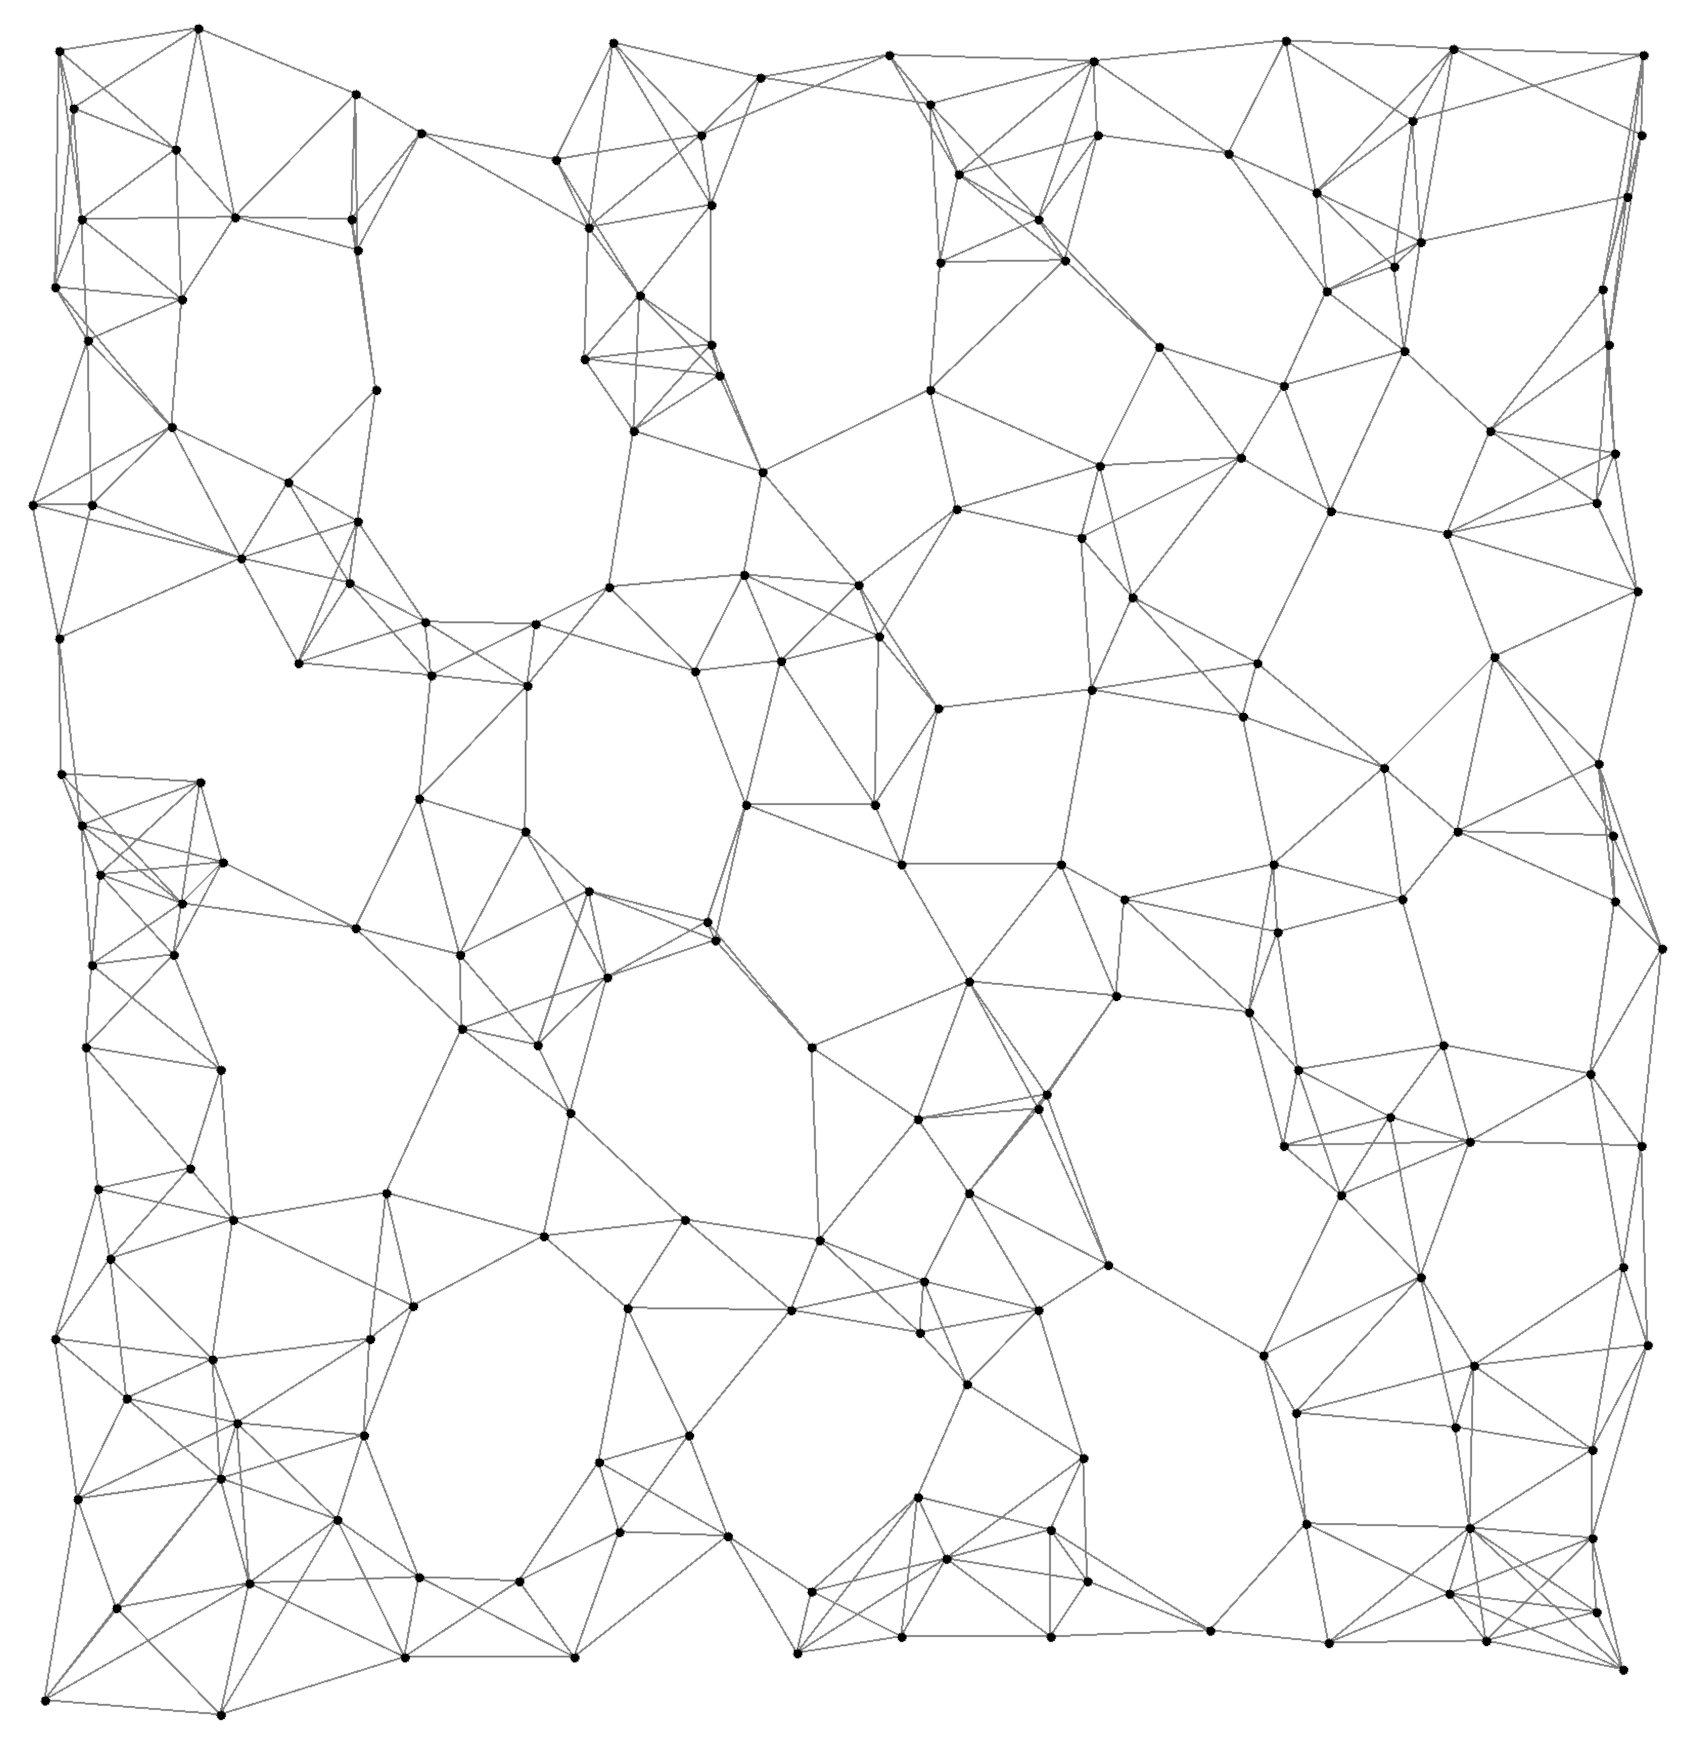
\includegraphics[width=0.25\textwidth]{img/1-large.png}}
\fbox{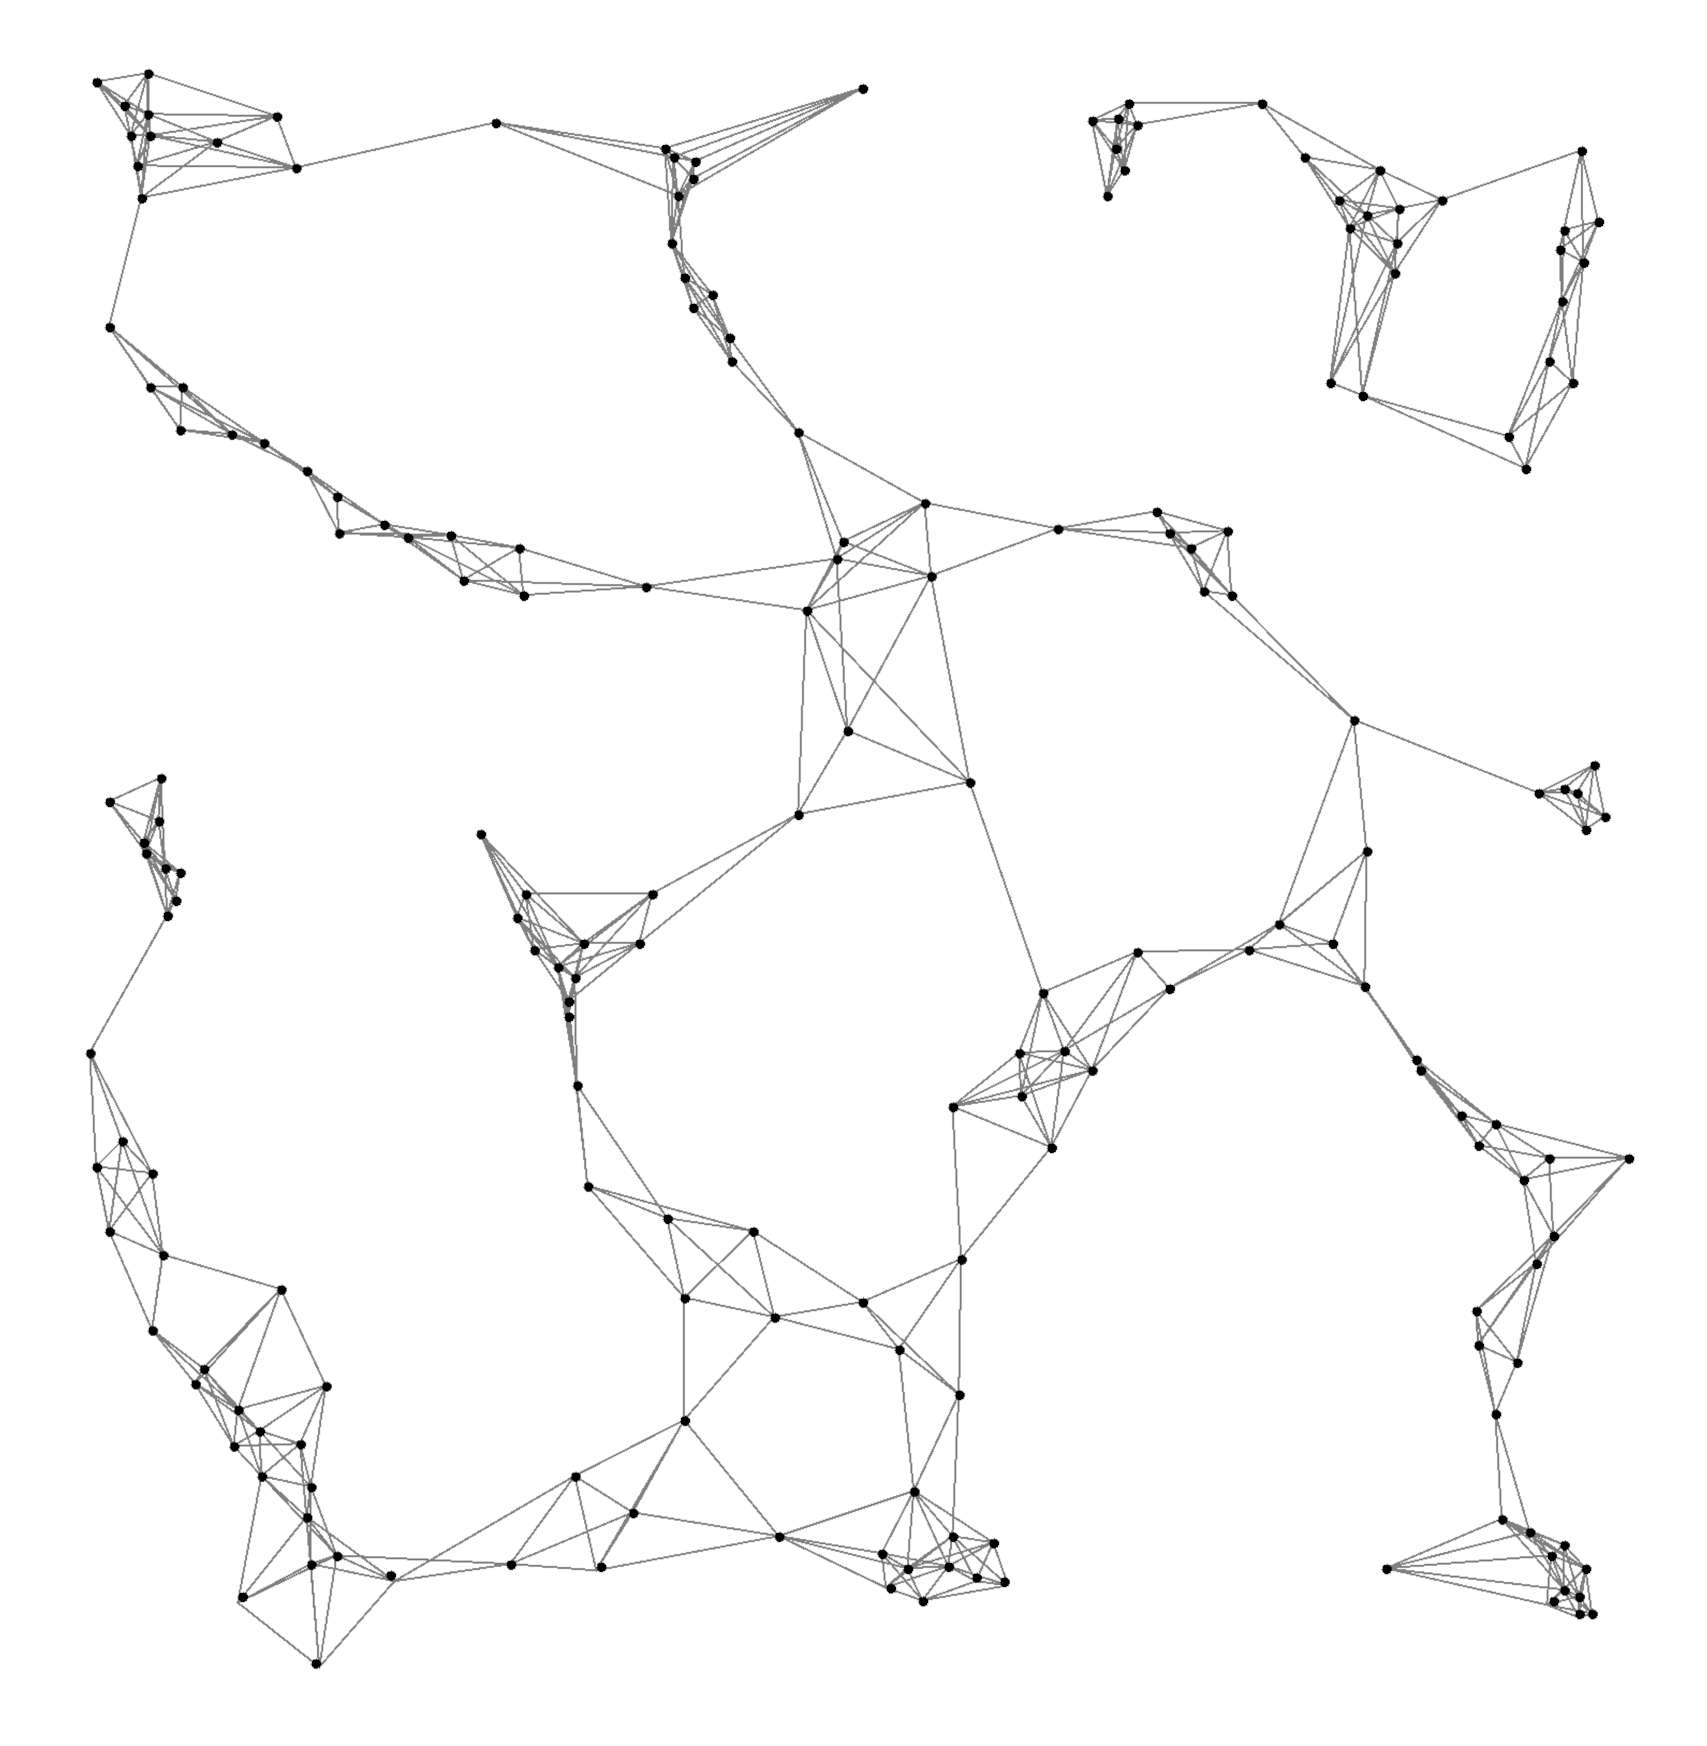
\includegraphics[width=0.25\textwidth]{img/3-large.png}}
\fbox{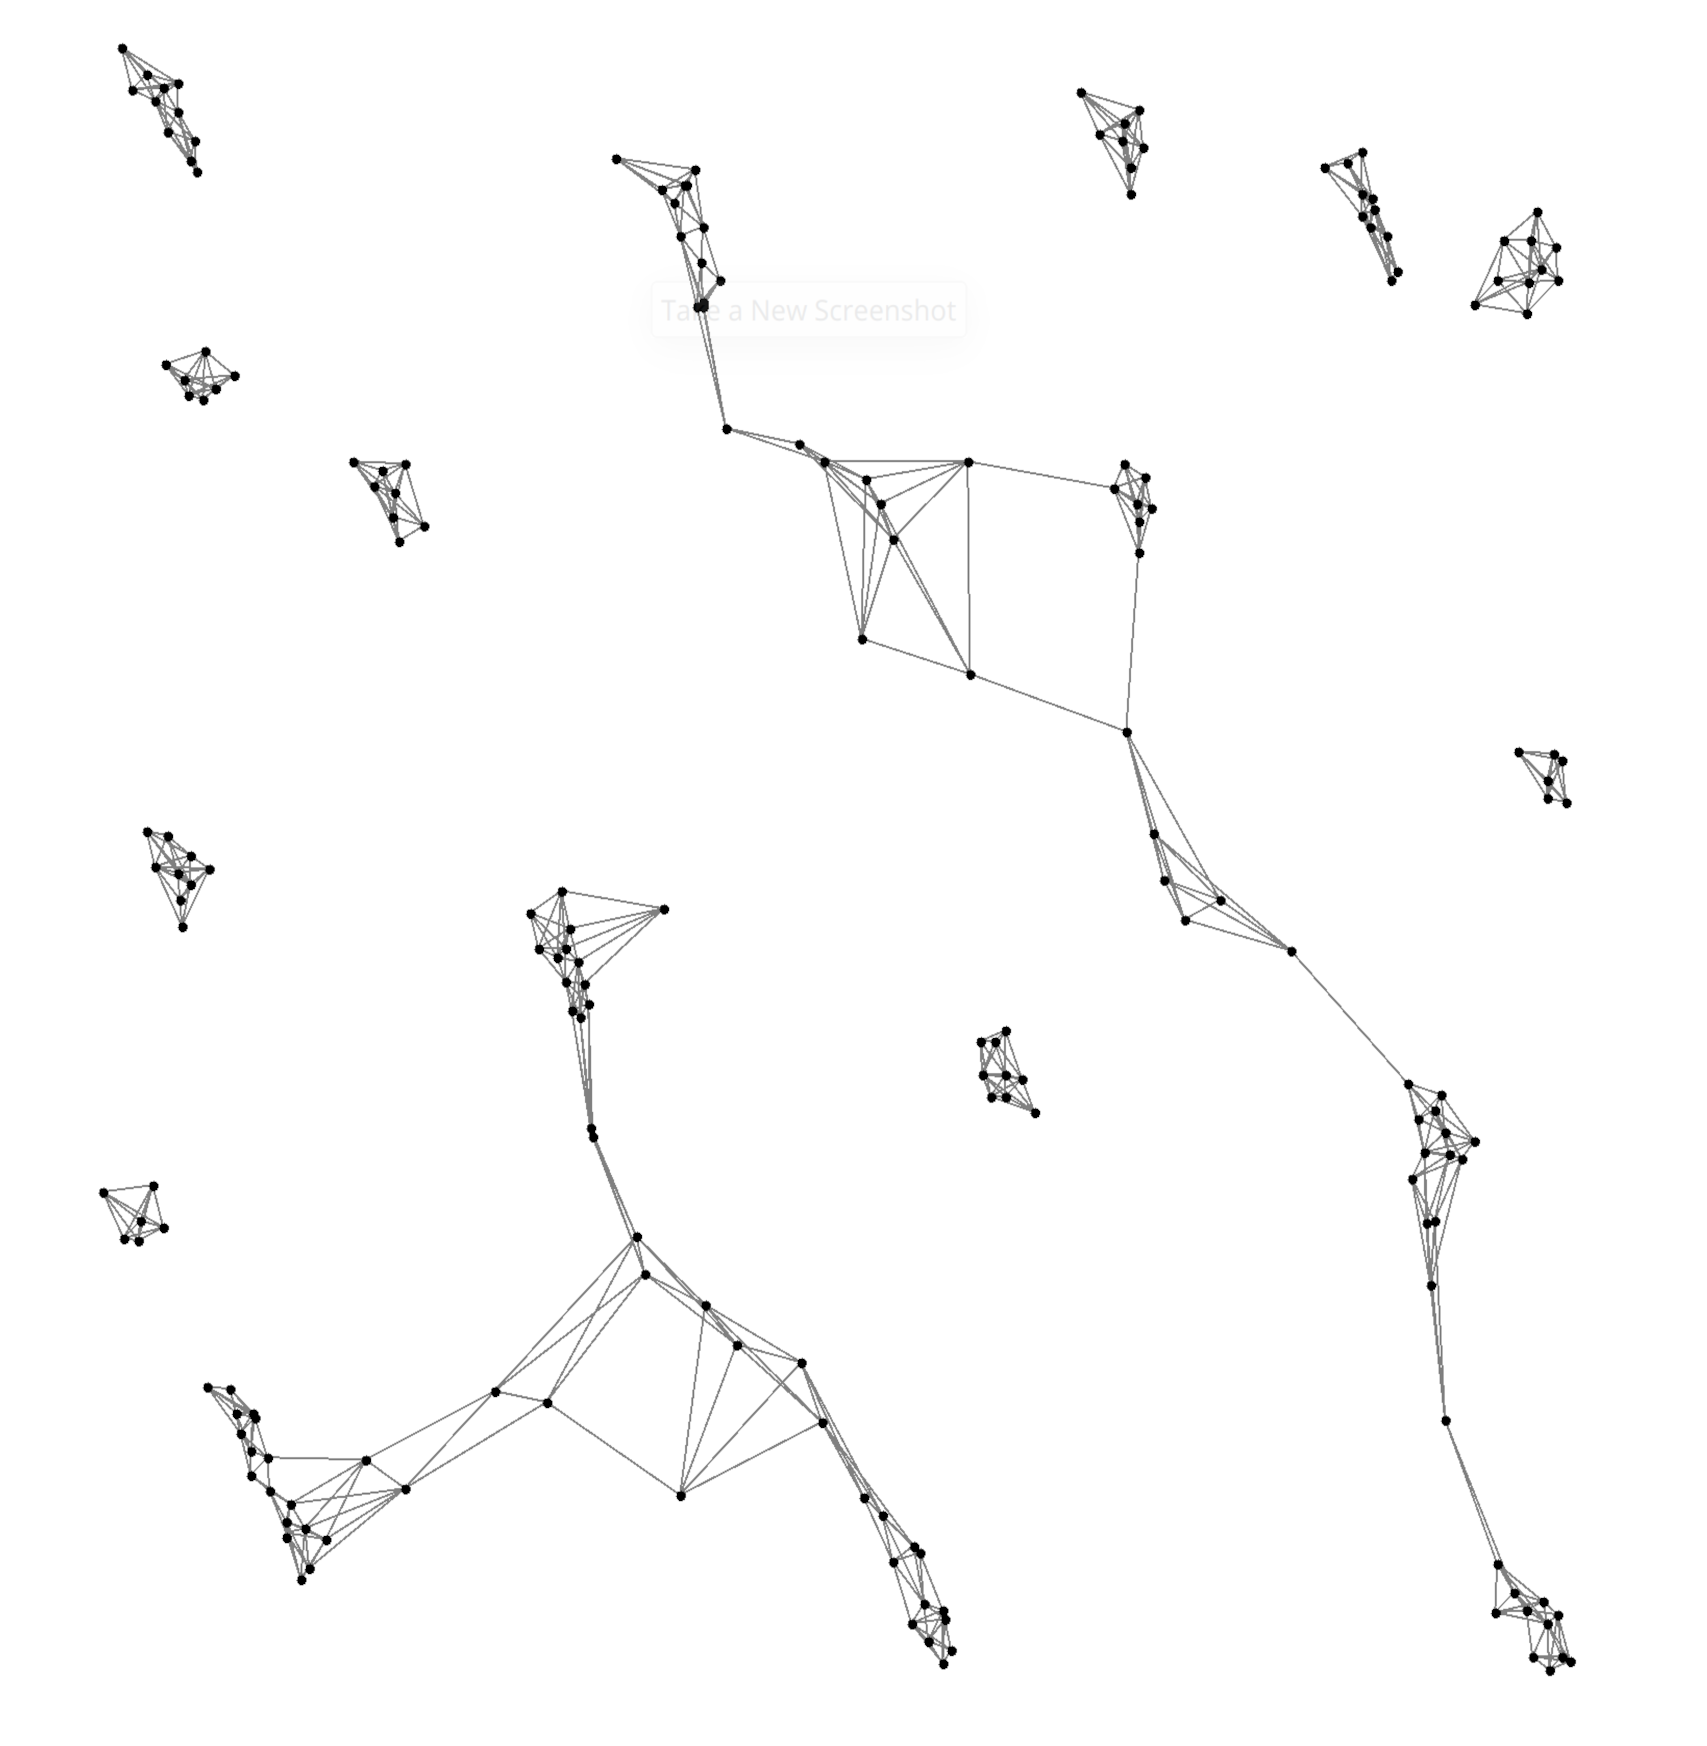
\includegraphics[width=0.25\textwidth]{img/4-large.png}}
\end{frame}

\begin{frame}{Conclusion}
\begin{exampleblock}{Wrap Up}
	\begin{itemize}
		\item CMARL is a prominent research area in RL
		\item We presented ScaRLib, a framework for the development of CMARL systems
		\item It supports the definition of different training modes (DTDE or CTDE) and it is possible to express the main components of a learning system (e.g., reward function, dataset, etc.)
		\item We exemplify the usage of ScaRLib with a flocking experiment
	\end{itemize}
\end{exampleblock}
\begin{alertblock}{Future works}
	\begin{itemize}
		\item Improve the DSL with more components
		\item Implement different state-of-the-art algorithms
		\item Integrate with other simulators (e.g., Gazebo or Webots)
	\end{itemize}
\end{alertblock}
\end{frame}

\begin{frame}{}
\centering
\Huge{Thank you!}

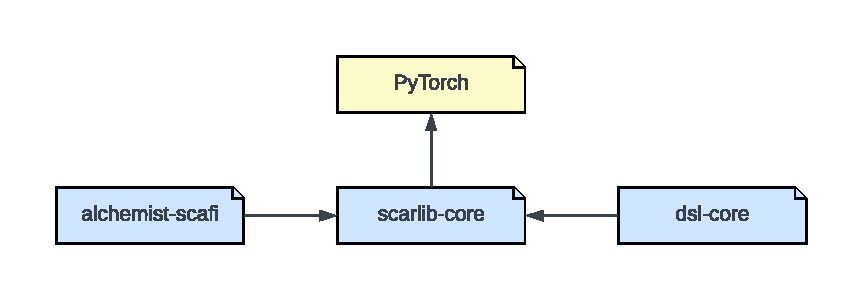
\includegraphics[width=0.3\textwidth]{img/scarlib-modules.pdf}
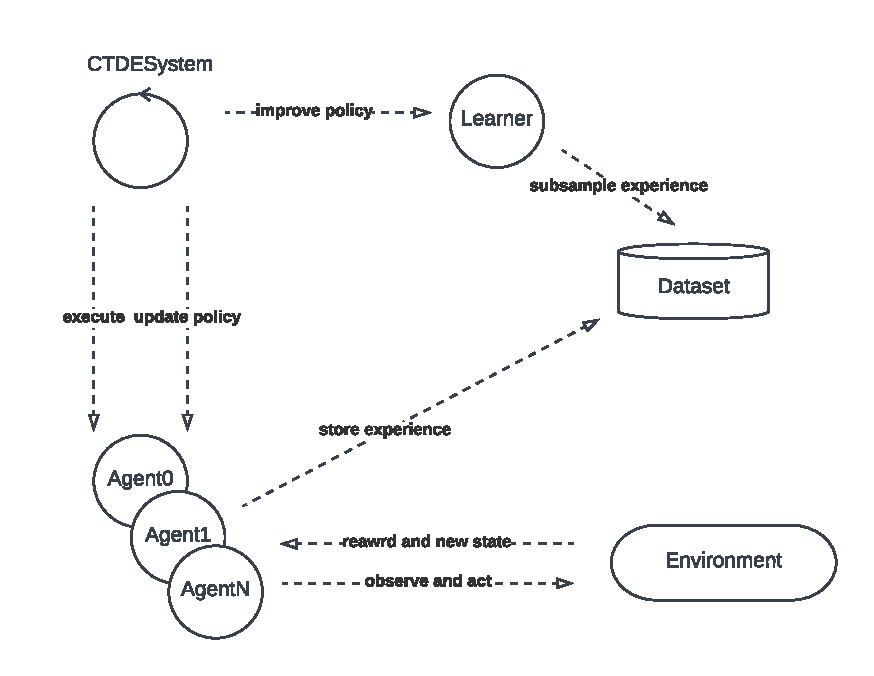
\includegraphics[width=0.3\textwidth]{img/ctdesystem.pdf}
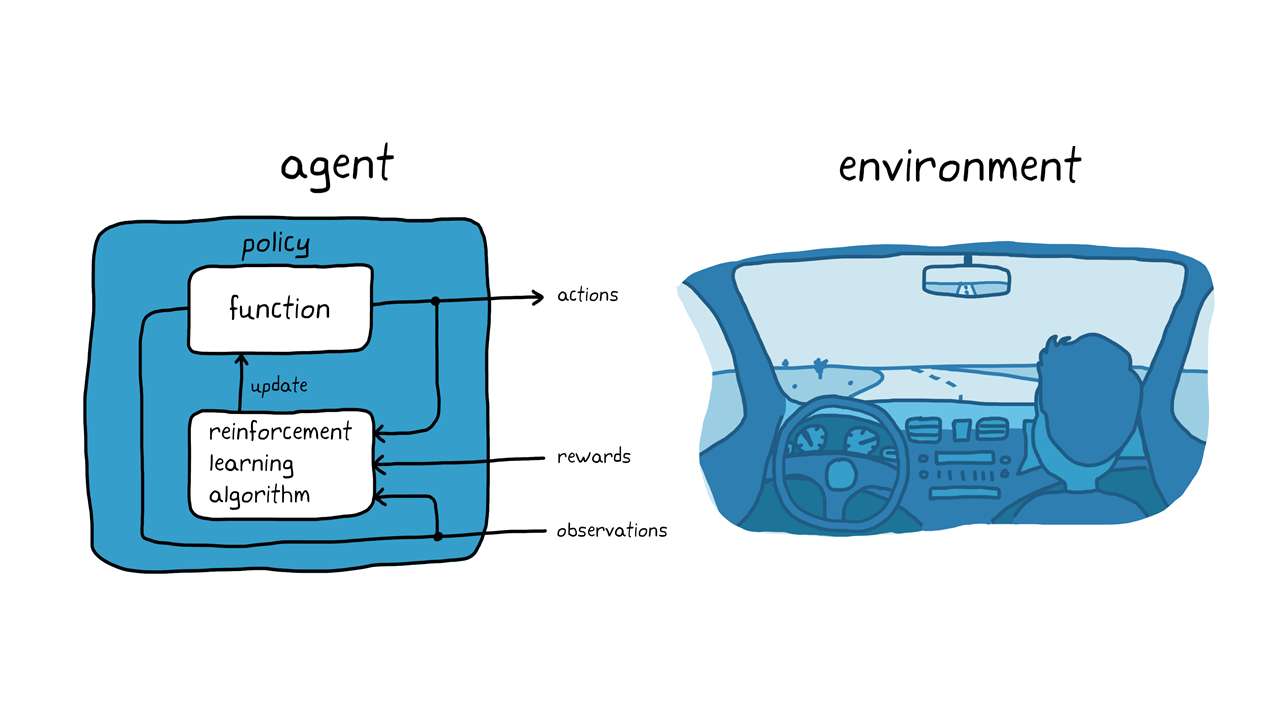
\includegraphics[width=0.3\textwidth]{img/simple-rl.png}

\fbox{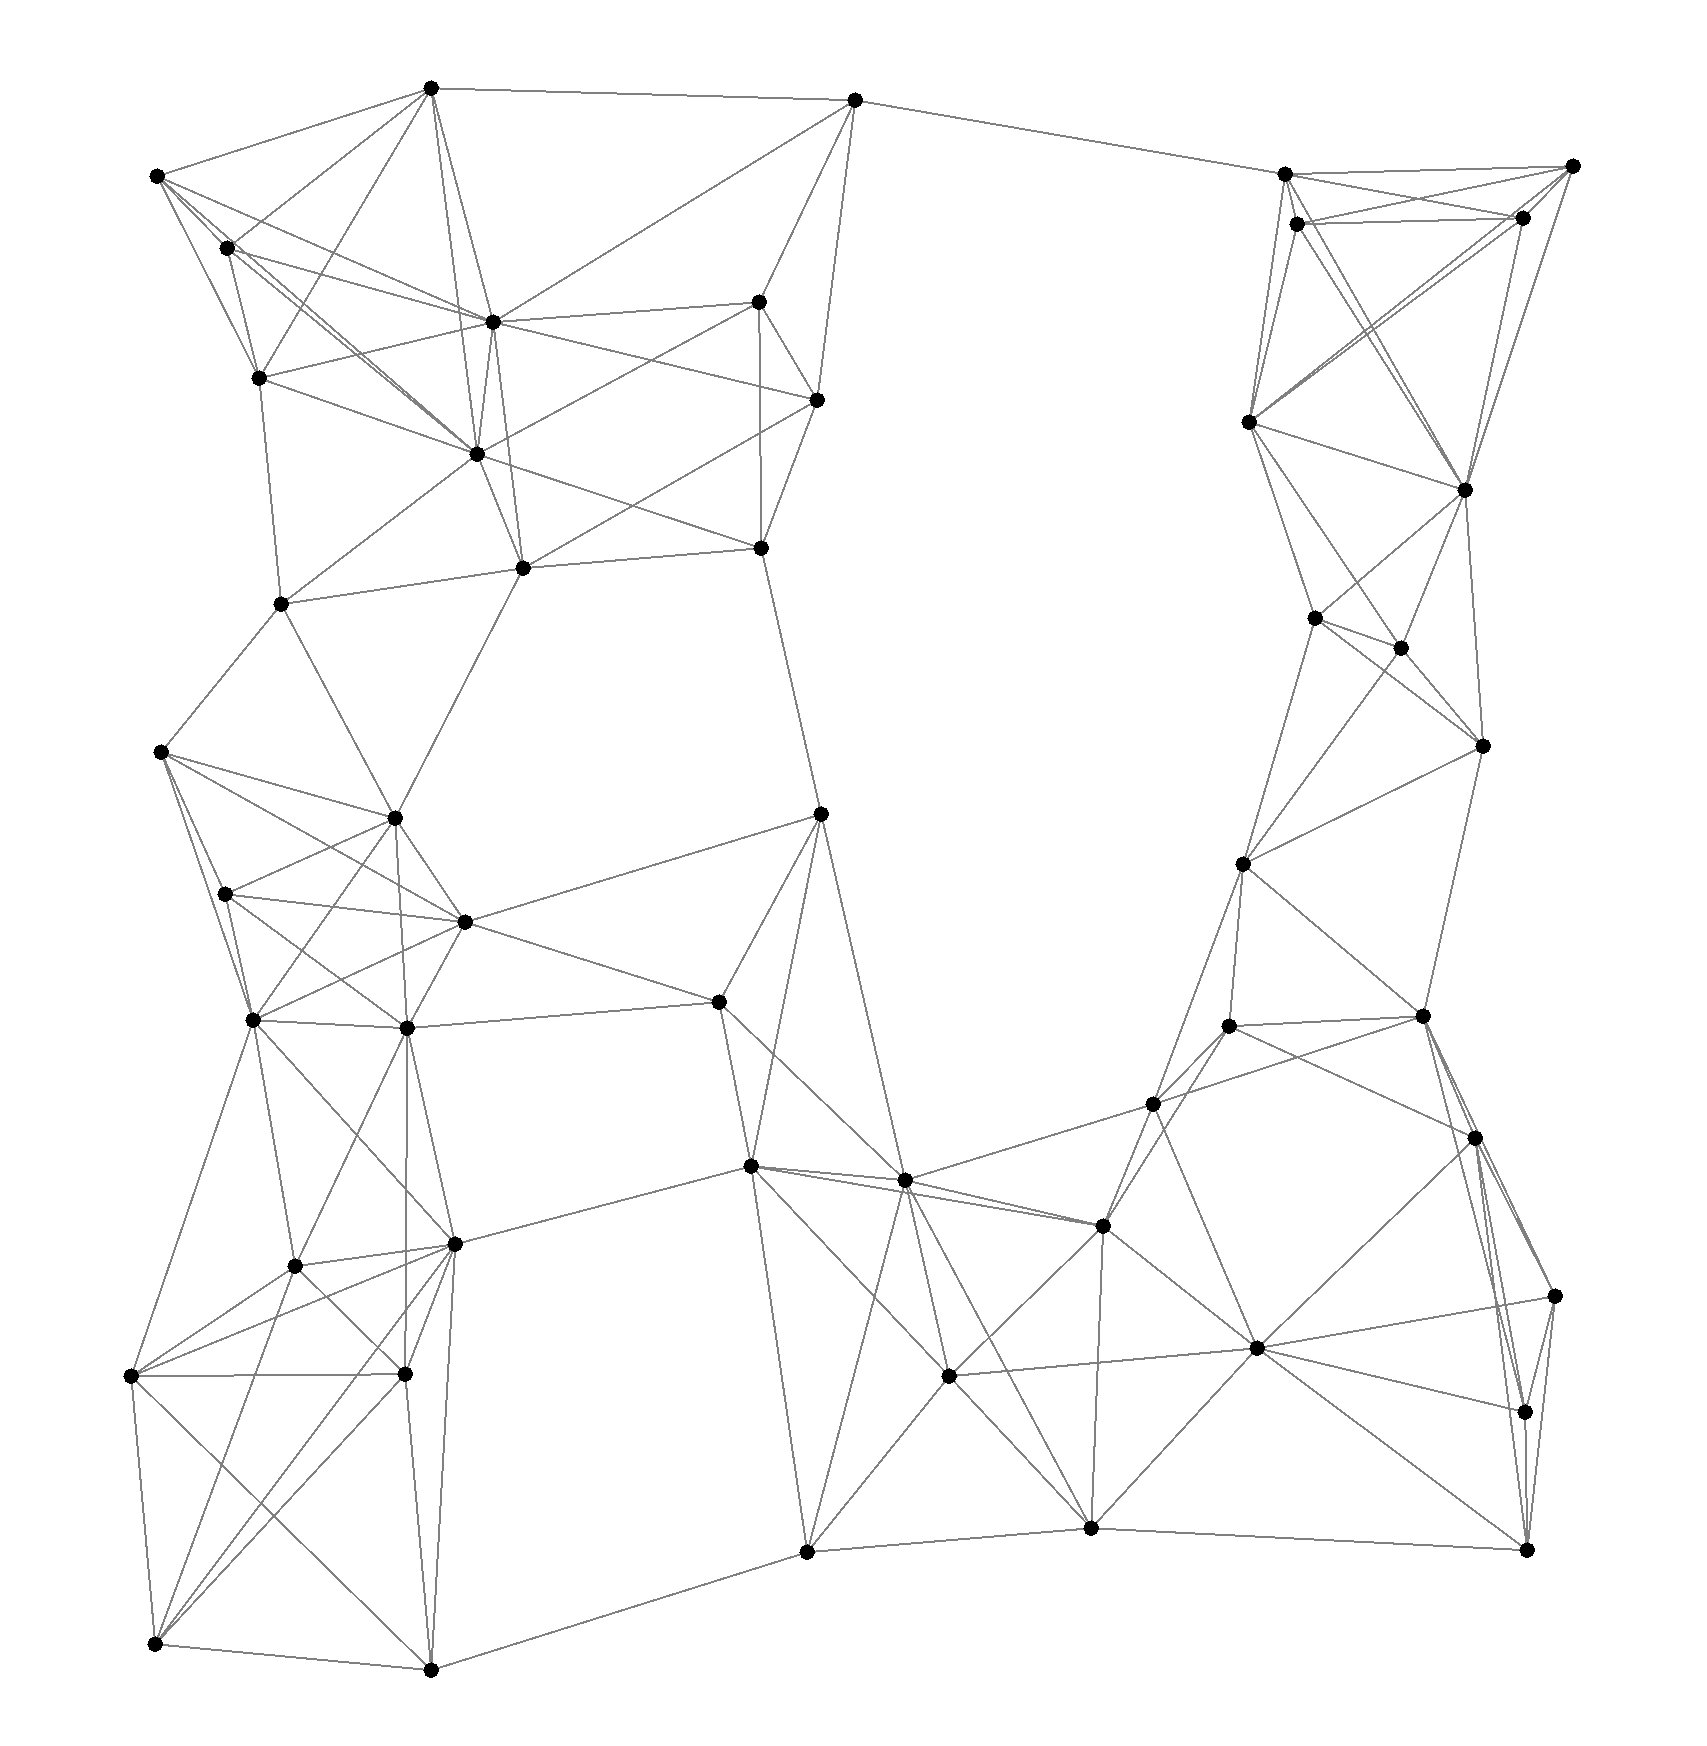
\includegraphics[width=0.15\textwidth]{img/1.png}}
\fbox{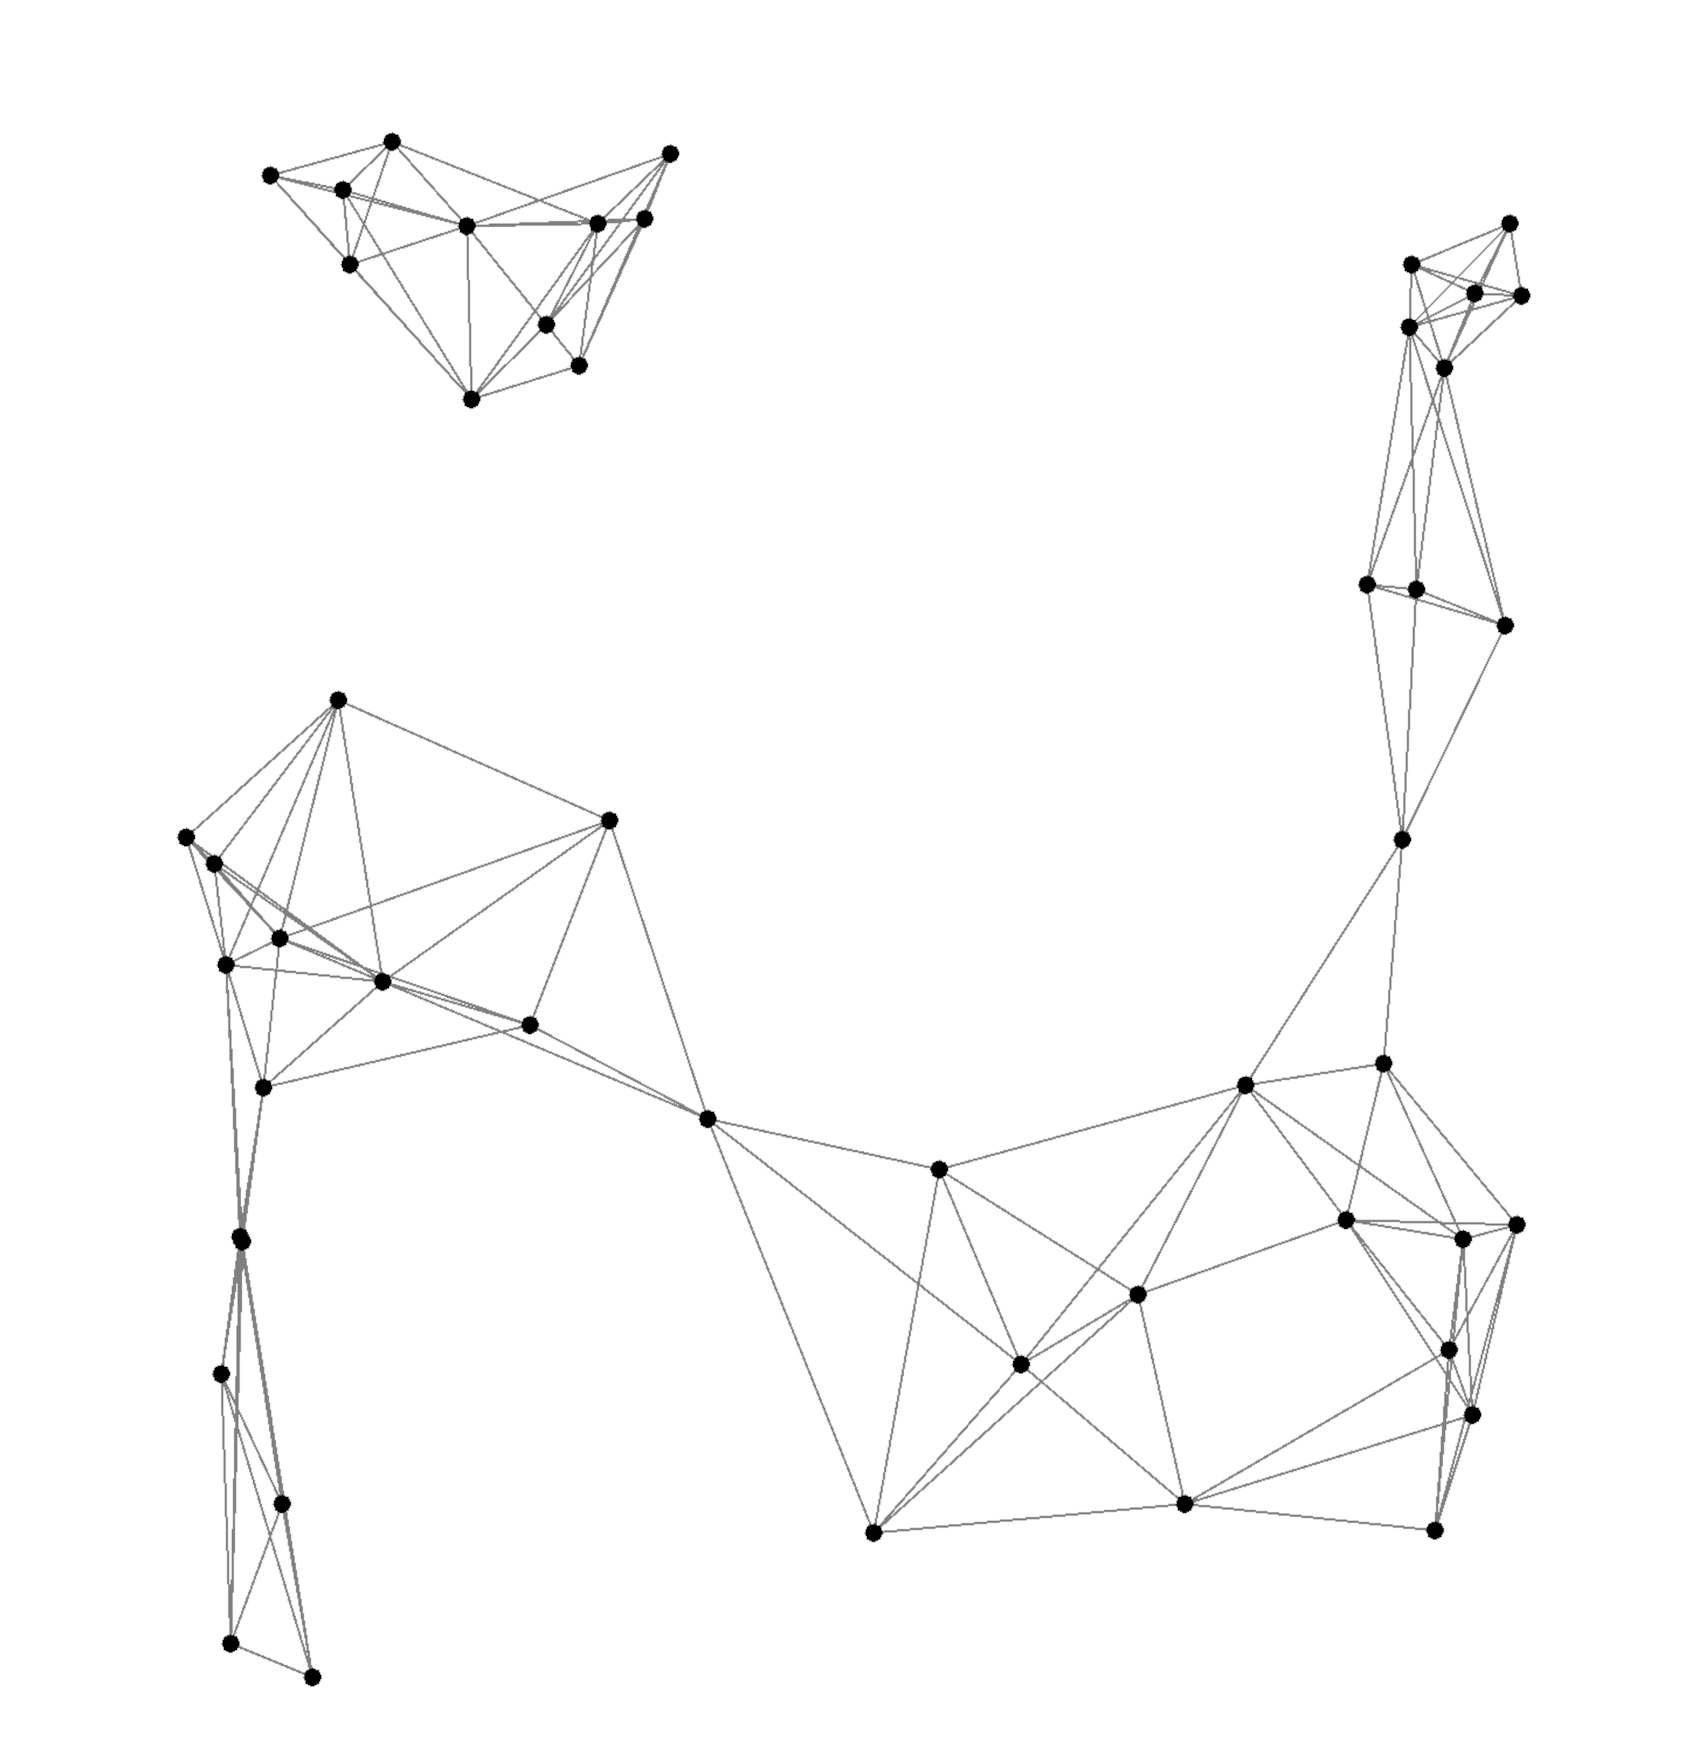
\includegraphics[width=0.15\textwidth]{img/4.png}}
\fbox{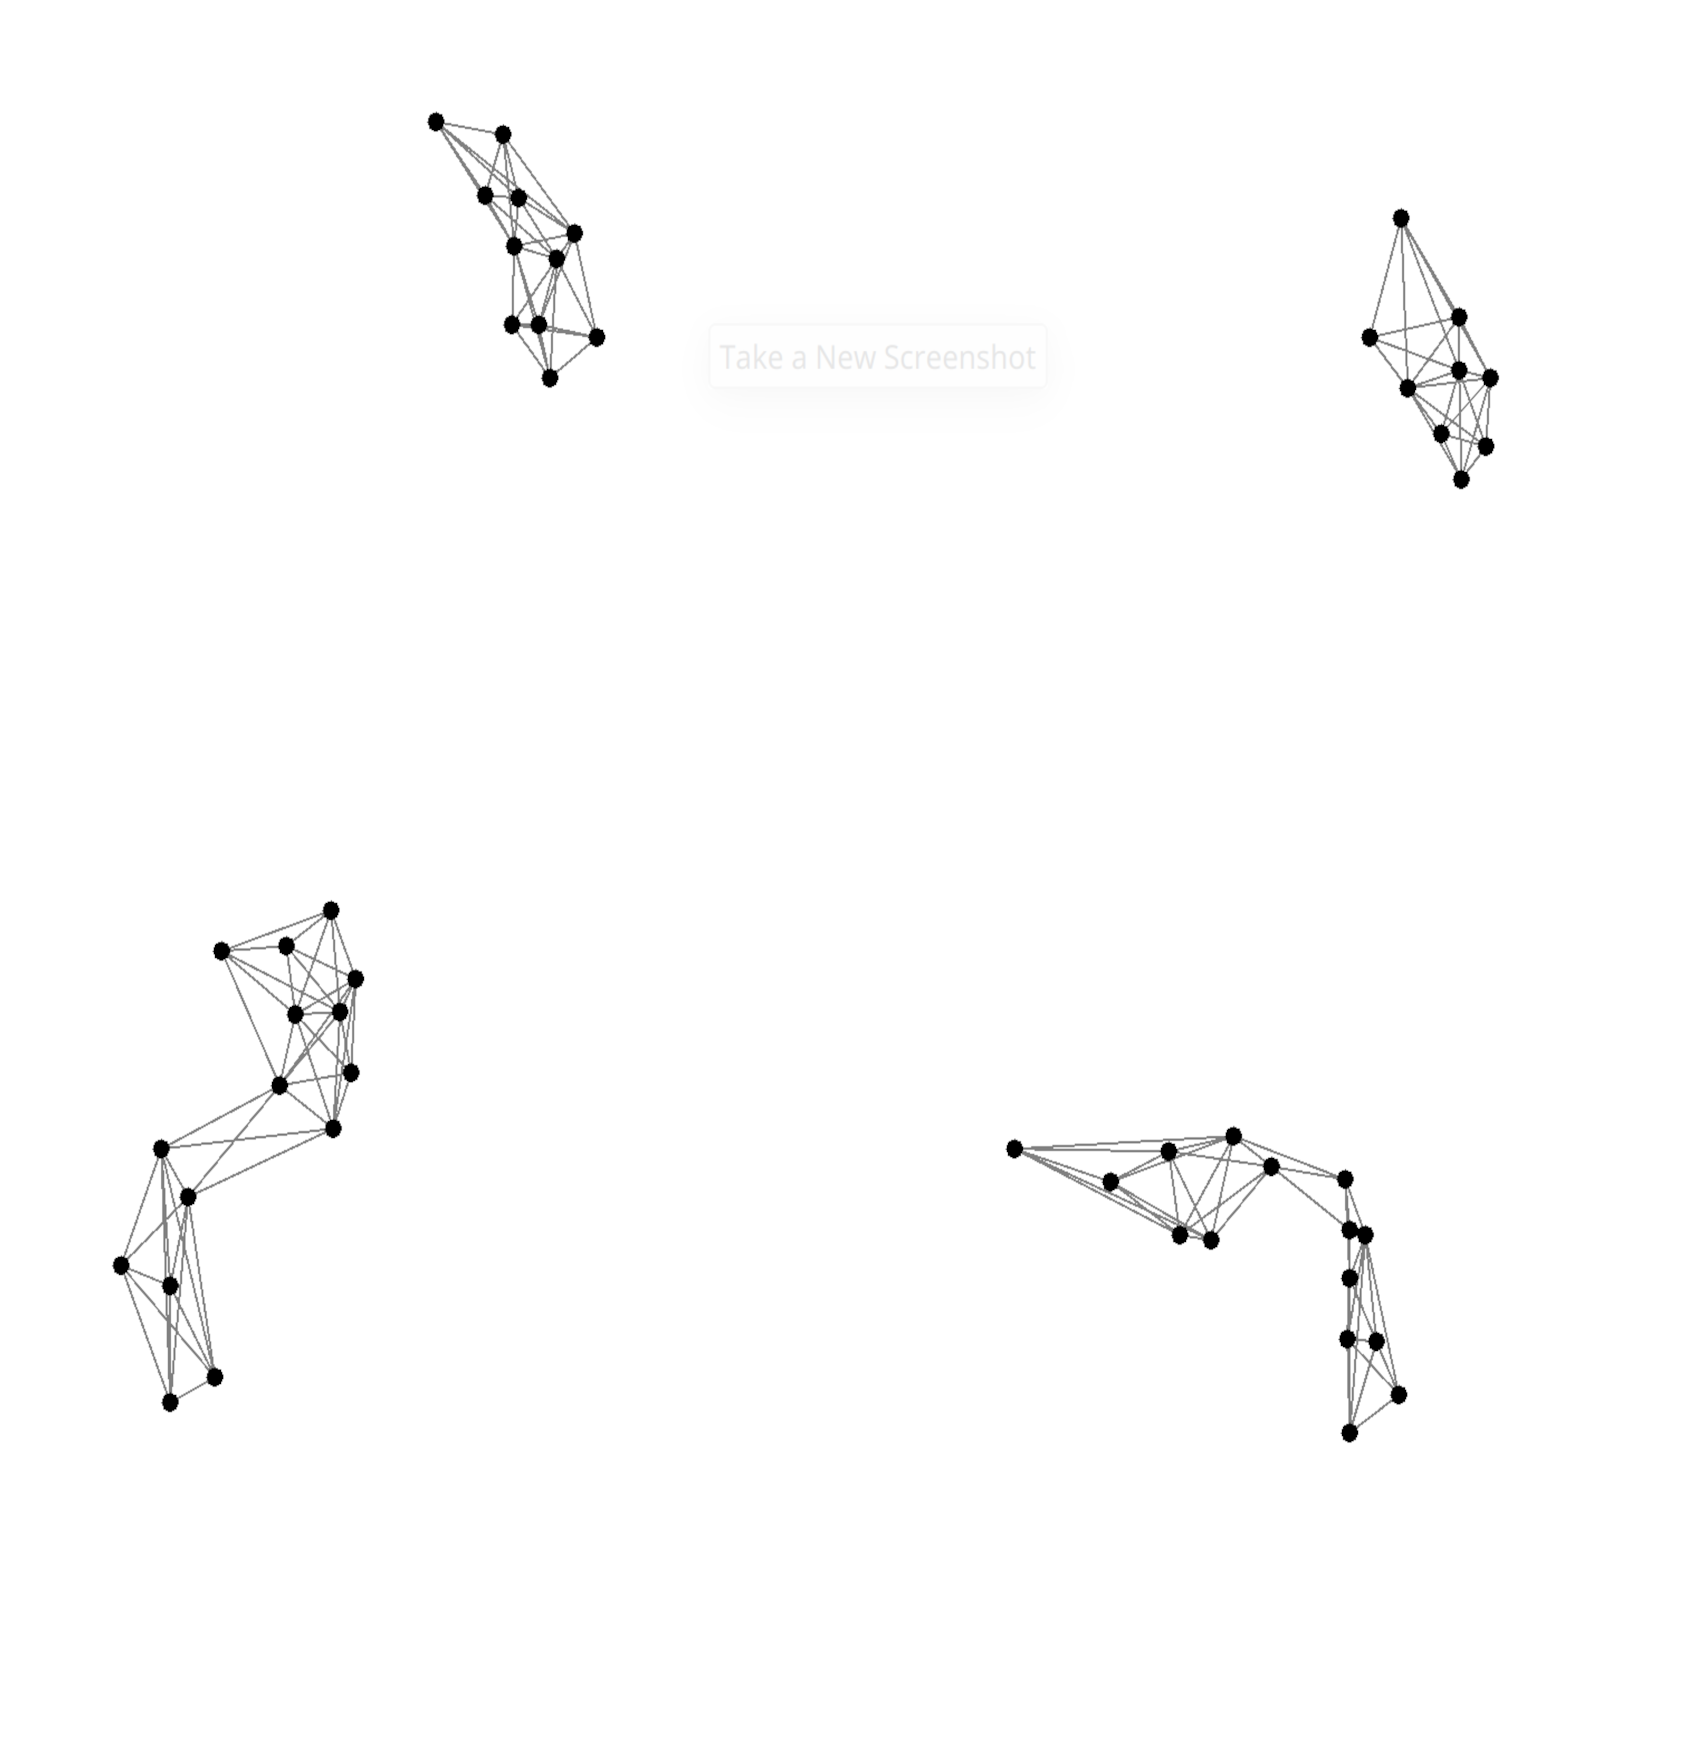
\includegraphics[width=0.15\textwidth]{img/7.png}}


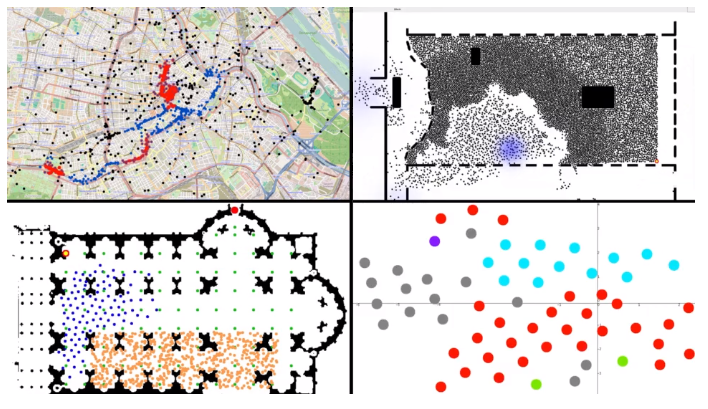
\includegraphics[width=0.3\textwidth]{img/alchemist}
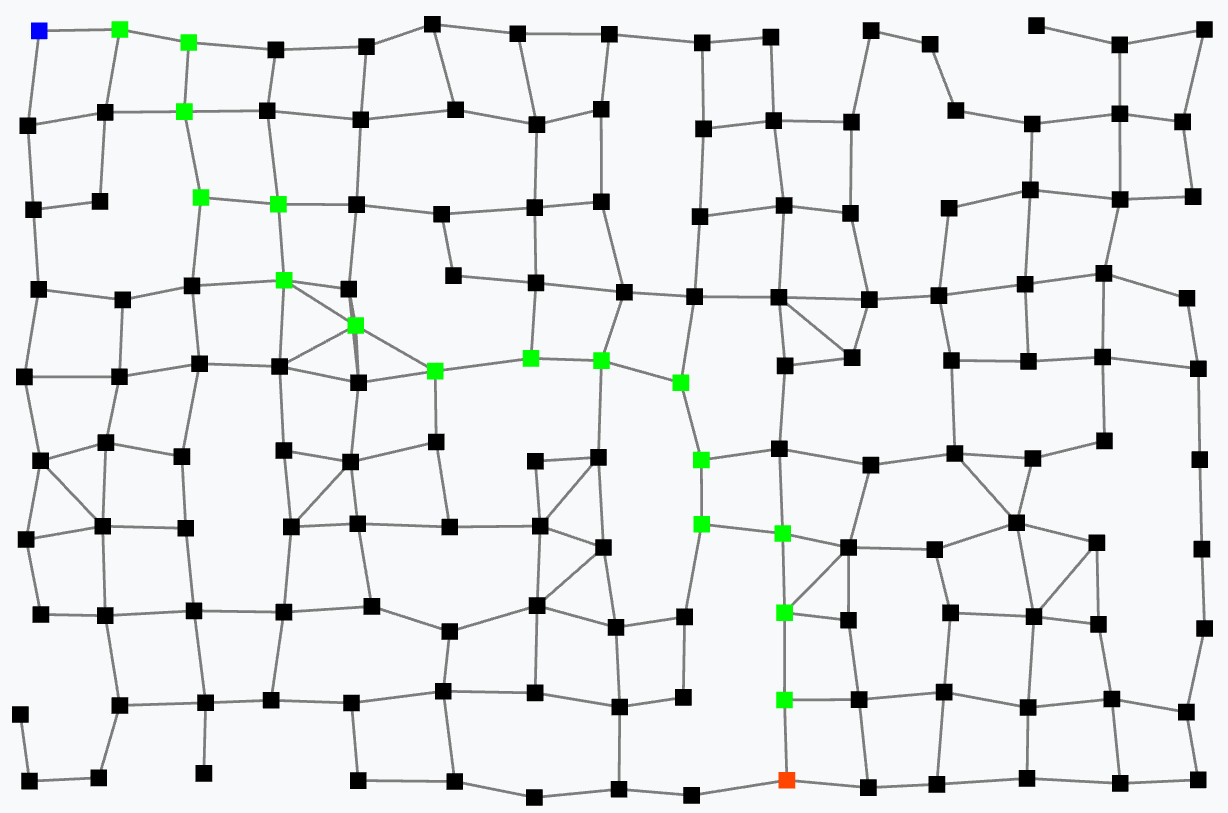
\includegraphics[width=0.3\textwidth]{img/channel.png}

\end{frame}
%===============================================================================
\section*{}
%===============================================================================

%/////////
\frame{\titlepage}
%/////////

%===============================================================================
\section*{\refname}
%===============================================================================


%%%%%%%%%%%%%%%%%%%%%%%%%%%%%%%%%%%%%%%%%%%%%%%%%%%%%%%%%%%%%%%%%%%%%%%%%%%%%%%%
\end{document}
%%%%%%%%%%%%%%%%%%%%%%%%%%%%%%%%%%%%%%%%%%%%%%%%%%%%%%%%%%%%%%%%%%%%%%%%%%%%%%%%
